\documentclass[10pt,a4paper]{article}

\usepackage[utf8]{inputenc}
\usepackage[T1]{fontenc}
\usepackage[brazilian]{babel}
\usepackage{lmodern}
\usepackage[margin=1.75cm,top=1.75cm,bottom=1.65cm]{geometry}
\usepackage{amsmath,amssymb,amsthm}
\usepackage{booktabs}
\usepackage{array}
\usepackage{colortbl}
\usepackage{xcolor}
\usepackage{graphicx}
\usepackage{tikz}
\usepackage{float}
\usepackage{caption}
\usepackage{fancyhdr}
\usepackage{listings}
\usepackage{parskip}
\usepackage[colorlinks=true,linkcolor=teal!70!black,urlcolor=blue!70!black,citecolor=teal!70!black]{hyperref}

\definecolor{ufopteal}{RGB}{0,105,112}
\definecolor{ufopbg}{RGB}{242,248,249}
\definecolor{codebg}{RGB}{246,248,250}
\definecolor{warnbg}{RGB}{255,248,236}
\definecolor{warnborder}{RGB}{190,120,30}

\pagestyle{fancy}
\fancyhf{}
\fancyhead[L]{\small\color{gray!70!black} BCC102 -- Matemática Discreta II \textbar{} CCO Explorer}
\fancyhead[R]{\small\color{gray!70!black} UFOP -- 2026.2}
\fancyfoot[C]{\small\color{gray!70!black} \thepage}
\renewcommand{\headrulewidth}{0.4pt}

\lstset{
  basicstyle=\ttfamily\footnotesize,
  backgroundcolor=\color{codebg},
  frame=single,
  rulecolor=\color{gray!40},
  breaklines=true,
  columns=fullflexible,
  xleftmargin=4pt,
  xrightmargin=4pt
}

\newsavebox{\ccobox}
\newenvironment{destaque}[1]{%
  \par\smallskip\noindent
  \begin{lrbox}{\ccobox}%
    \begin{minipage}{\dimexpr\linewidth-18pt\relax}%
      \textbf{\color{ufopteal}#1}\par\smallskip
}{%
    \end{minipage}%
  \end{lrbox}%
  \begin{tikzpicture}
    \node[fill=ufopbg, draw=ufopteal, line width=0.8pt, rounded corners=3pt, inner sep=8pt] {\usebox{\ccobox}};
  \end{tikzpicture}\par\smallskip
}

\newenvironment{alerta}[1]{%
  \par\smallskip\noindent
  \begin{lrbox}{\ccobox}%
    \begin{minipage}{\dimexpr\linewidth-18pt\relax}%
      \textbf{\color{warnborder}#1}\par\smallskip
}{%
    \end{minipage}%
  \end{lrbox}%
  \begin{tikzpicture}
    \node[fill=warnbg, draw=warnborder, line width=0.8pt, rounded corners=3pt, inner sep=8pt] {\usebox{\ccobox}};
  \end{tikzpicture}\par\smallskip
}

\setcounter{tocdepth}{2}

\captionsetup{font=small, labelfont=bf}

\begin{document}

% ============================================================================
% CABECALHO / CAPA COMPACTA CIENTIFICO-TECNICA
% ============================================================================
\thispagestyle{empty}
\begin{center}
  {\large\textbf{UNIVERSIDADE FEDERAL DE OURO PRETO (UFOP)}}\\[2pt]
  {\normalsize Instituto de Ciências Exatas e Biológicas (ICEB) -- Departamento de Computação (DECOM)}\\[10pt]
  \textcolor{ufopteal}{\rule{\linewidth}{1.6pt}}\\[14pt]
  {\LARGE\bfseries\color{ufopteal} CCO Explorer}\\[6pt]
  {\Large\bfseries Aplicações de Matemática Discreta na Análise de Redes Vasculares}\\[10pt]
  {\normalsize Relatório Científico-Técnico -- Trabalho Prático (TP)}\\
  {\normalsize BCC102 -- Matemática Discreta II \textbar{} Período: 2026.2}\\[12pt]
  \textcolor{ufopteal}{\rule{\linewidth}{0.8pt}}
\end{center}

\vspace{6pt}
\begin{center}
  \begin{tabular}{ll}
    \textbf{Linguagem principal:} & C++20 (compilado com CMake no ambiente reprodutível \texttt{devenv}) \\
    \textbf{Scripts auxiliares:} & Python 3 (biblioteca padrão: verificação cruzada, figuras TikZ e empacotamento) \\
    \textbf{Trilha eletiva (B1):} & \textbf{Trilha 1 -- Algoritmo de Euclides e Teorema Chinês do Resto (TCR)} \\
    \textbf{Integrantes do grupo:} & \textit{Preencher nomes completos e matrículas antes da submissão final} \\
    \textbf{Data:} & Novembro / Dezembro de 2026 \\
  \end{tabular}
\end{center}

\begin{destaque}{Resumo Executivo}
Este trabalho apresenta o projeto, a modelagem matemática, a implementação em C++20 e a verificação
reprodutível do programa \textbf{CCO Explorer}, desenvolvido para analisar seis modelos tridimensionais
reais de árvores vasculares geradas pelo método \textit{Constrained Constructive Optimization} (CCO),
com $N_{\mathrm{term}} \in \{16, 32, 64, 128, 256, 512\}$ segmentos terminais. Articulando os quatro
eixos da ementa de BCC102 -- Teoria dos Números, Técnicas de Contagem, Relações de Recorrência e
Relações e suas Propriedades --, o programa extrai e valida integralmente os seis arquivos VTK,
calcula atributos geométricos 3D nas unidades originais, executa consultas determinísticas por
aritmética modular e pelo Teorema Chinês do Resto ($i \equiv 17 \pmod{20}$), verifica identidades
combinatórias e o Princípio da Inclusão--Exclusão sobre medianas geométricas em \texttt{Nterm128}
($|A \cup B| = 128 + 128 - 42 = 214$), deduz e valida recorrências exatas ($e_k = 32\cdot 2^k - 1$,
$b_k = 16\cdot 2^k - 1$, $v_k = 32\cdot 2^k$) e analisa a relação pai--filho $\mathcal{R}$, sua
função associada $p$, seu fecho transitivo $\mathcal{R}^+$ ($179$ pares em \texttt{Nterm016}), a
ordem parcial $\preceq$ ($317$ pares incomparáveis) e a relação de equivalência modular $\sim$. Todos
os sete testes mínimos de aceitação (T1--T7) foram validados em C++ via \texttt{CTest} e confirmados
por verificação cruzada independente em Python.
\end{destaque}

\tableofcontents
\vspace{4pt}
\hrule
\vspace{6pt}

% ============================================================================
% 1. INTRODUCAO E OBJETIVO
% ============================================================================
\section{Introdução e Objetivo}

O método \textit{Constrained Constructive Optimization} (CCO) é amplamente empregado na modelagem
computacional de redes vasculares artificiais tridimensionais sujeitas a restrições geométricas e
fisiológicas de perfusão~\cite{karch1999cco}. Embora a geração dessas árvores envolva otimização
geométrica e equações hemodinâmicas, a estrutura resultante é uma rede discreta de conexões
orientadas entre pontos tridimensionais e segmentos tubulares caracterizados por raios escalares.

O objetivo deste Trabalho Prático consiste em projetar e implementar o \textbf{CCO Explorer}, um
sistema reprodutível de linha de comando em C++20 que lê os seis arquivos VTK fornecidos, valida
rigorosamente sua integridade estrutural e produz análises matemáticas fundamentadas nos quatro
eixos de \textbf{BCC102 -- Matemática Discreta II}:
\begin{enumerate}
  \item \textbf{Modelagem discreta e validação (Módulo A):} extração de pontos, segmentos e raios,
        incorporação da geometria euclidiana 3D (comprimentos e pontos médios) e classificação
        topológica dos pontos apenas com vetores, matrizes, laços e contadores elementares.
  \item \textbf{Teoria dos Números (Módulo B):} agrupamento determinístico por congruência módulo
        $m = 7$, verificação de partição, Princípio da Casa dos Pombos e implementação da
        \textbf{Trilha 1 (Algoritmo de Euclides e Teorema Chinês do Resto)}.
  \item \textbf{Contagem e Relações de Recorrência (Módulo C):} invariantes estruturais por dupla
        contagem, combinações $\binom{T}{2}$, princípio multiplicativo $B \times T$, Inclusão--Exclusão
        sobre atributos 3D e resolução de recorrências por iteração e equação característica.
  \item \textbf{Relações e suas Propriedades (Módulo D):} formalização da relação pai--filho
        $\mathcal{R}$, matriz booleana $32 \times 32$ para \texttt{Nterm016}, análise de propriedades
        e da inversa $\mathcal{R}^{-1}$, função pai $p$, fecho transitivo iterativo $\mathcal{R}^+$,
        ordem parcial $\preceq$ e relação de equivalência modular $\sim$.
\end{enumerate}

Seguindo as restrições pedagógicas do enunciado, não foram empregadas estruturas especializadas de
Estruturas de Dados I (como nós encadeados do tipo \texttt{TreeNode} ou bibliotecas externas de
grafos), nem bibliotecas externas de leitura VTK: toda a modelagem e as transformações matemáticas
foram implementadas explicitamente em C++20 com vetores, matrizes booleanas, laços e funções puras.

% ============================================================================
% 2. DESCRICAO DOS DADOS E PREMISSAS
% ============================================================================
\section{Descrição dos Dados e Premissas}

O conjunto de entrada disponibilizado na pasta \texttt{dados/} contém seis arquivos no formato legado
VTK ASCII (\texttt{DATASET POLYDATA}), nomeados \texttt{tree3D\_Nterm016.vtk} até
\texttt{tree3D\_Nterm512.vtk}, acompanhados de imagens PNG ilustrativas de renderização tubular.
Cada arquivo VTK organiza-se em três seções relevantes:
\begin{itemize}
  \item \texttt{POINTS $|V|$ float}: coordenadas tridimensionais $(x_v, y_v, z_v)$ dos pontos,
        indexados implicitamente por $v \in V = \{0, 1, \dots, |V|-1\}$;
  \item \texttt{LINES $|E|$ $3|E|$}: registros da forma \texttt{2 u v}, definindo segmentos
        orientados da extremidade proximal $u$ para a distal $v$, recebendo identificadores
        $i \in \{0, 1, \dots, |E|-1\}$ conforme a ordem de apresentação;
  \item \texttt{CELL\_DATA $|E|$} (\texttt{scalars raio float}): atributo escalar de raio $r_i$
        associado univocamente ao segmento $s_i$ na mesma ordenação de \texttt{LINES}.
\end{itemize}

\begin{alerta}{Premissas de Rigor sobre Unidades, Entidades e Apoio Visual}
\textbf{(i) Unidades originais:} nenhum cabeçalho VTK declara unidades físicas (metros ou milímetros);
todas as grandezas geométricas ($\ell_i$, $M_i$, $r_i$) são preservadas nas unidades numéricas
originais dos arquivos.
\textbf{(ii) Distinção conceitual:} distinguem-se rigorosamente \emph{pontos} ($v \in V$),
\emph{segmentos} ($s_i = (u_i, v_i) \in E$) e \emph{terminais} ($t \in V$ com grau de saída nulo).
\textbf{(iii) Apoio visual:} as imagens PNG da Figura~\ref{fig:modelos_png} servem exclusivamente como
ilustração qualitativa da geometria 3D; todos os valores numéricos deste relatório foram calculados
diretamente a partir dos arquivos VTK pelo executável \texttt{cco\_explorer}.
\end{alerta}

\begin{figure}[H]
  \centering
  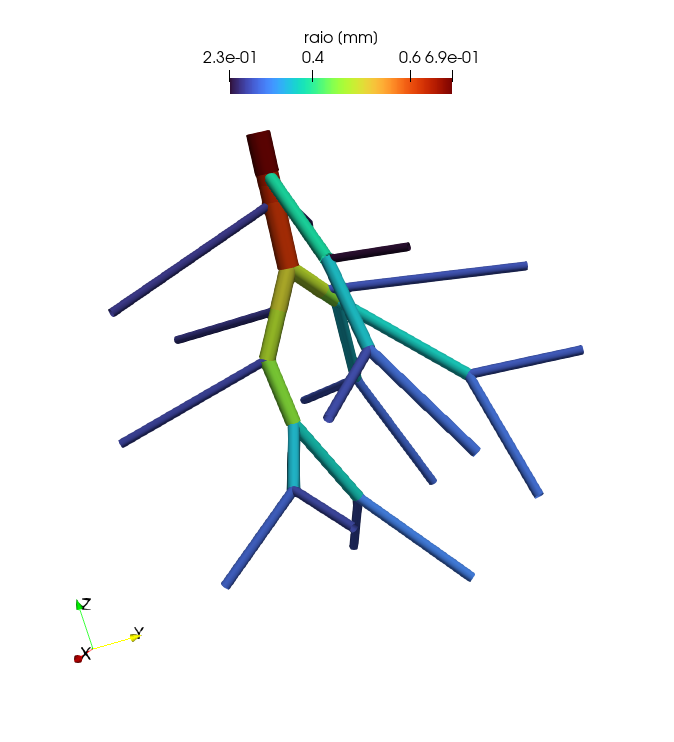
\includegraphics[width=0.31\textwidth]{../dados/tree3D_Nterm016_tube.png}\hspace{1.2cm}
  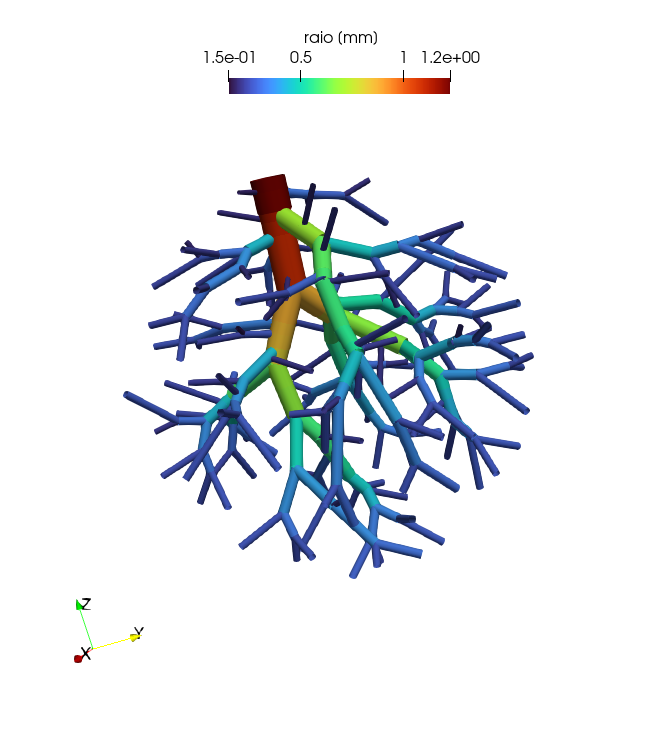
\includegraphics[width=0.31\textwidth]{../dados/tree3D_Nterm128_tube.png}
  \caption{Apoio visual dos modelos tridimensionais fornecidos: \texttt{Nterm016} (esquerda, $16$ terminais e $31$ segmentos) e \texttt{Nterm128} (direita, $128$ terminais e $255$ segmentos). Imagens originais da coleção usadas apenas como ilustração.}
  \label{fig:modelos_png}
\end{figure}

% ============================================================================
% 3. MODULO A -- MODELAGEM DISCRETA E VALIDACAO
% ============================================================================
\section{Módulo A -- Modelagem Discreta e Validação dos Dados}

\subsection{Extração, Geometria 3D e Validação (A1--A3)}

O módulo \texttt{vtk\_parser} lê o cabeçalho (\texttt{\# vtk DataFile}, \texttt{ASCII},
\texttt{DATASET POLYDATA}) e percorre as seções \texttt{POINTS}, \texttt{LINES} e \texttt{CELL\_DATA}.
Para cada segmento $s_i$ com extremos $P_{u_i} = (x_u, y_u, z_u)$ e $P_{v_i} = (x_v, y_v, z_v)$, são
calculados o comprimento euclidiano tridimensional e o ponto médio:
\begin{equation}
  \ell_i = \sqrt{(x_v - x_u)^2 + (y_v - y_u)^2 + (z_v - z_u)^2}, \qquad
  M_i = \left(\frac{x_u + x_v}{2},\; \frac{y_u + y_v}{2},\; \frac{z_u + z_v}{2}\right).
\end{equation}

Na validação automática (item A3), o programa verifica: (i) correspondência exata entre as
quantidades declaradas e lidas de pontos, linhas e dados de célula; (ii) total de inteiros em
\texttt{LINES} igual a $3|E|$ e aridade $2$ em cada linha; (iii) existência de todos os índices
$u_i, v_i \in \{0, \dots, |V|-1\}$ sem laços próprios ($u_i \neq v_i$); (iv) correspondência
biunívoca de um raio positivo e finito por segmento; e (v) ausência de valores excedentes após
\texttt{CELL\_DATA}. Um teste unitário negativo dedicado confirma que um VTK corrompido (referenciando
índice inexistente) é rejeitado com \texttt{validation.ok = false}.

\subsection{Identificação Estrutural dos Pontos e Tabela Consolidada (A4)}

Por meio de laços simples sobre $E$, contabilizam-se o grau de entrada $\deg^-(v)$ e o grau de saída
$\deg^+(v)$ de cada ponto $v \in V$. Em \textbf{todos os seis arquivos}, a verificação empírica
confirmou sem exceção exatamente três classes disjuntas de vértices:
\begin{itemize}
  \item \textbf{Entrada única:} somente o ponto $0$ apresenta $(\deg^-(0), \deg^+(0)) = (0, 1)$,
        confirmando que o ponto de entrada \emph{não} é uma bifurcação;
  \item \textbf{Bifurcações ($B$):} pontos internos com $(\deg^-(v), \deg^+(v)) = (1, 2)$;
  \item \textbf{Terminais ($T$):} pontos distais com $(\deg^-(v), \deg^+(v)) = (1, 0)$.
\end{itemize}
Nenhum ponto anômalo foi detectado em qualquer modelo. A Tabela~\ref{tab:consolidada} consolida
as contagens estruturais (em concordância exata com a Tabela 1 do enunciado) e as medidas
geométricas 3D extraídas, também exportadas em \texttt{resultados/resumo\_consolidado.csv} e nos
arquivos individuais por segmento em \texttt{resultados/segmentos/}.

\begin{table}[H]
  \centering
  \caption{Tabela consolidada dos seis modelos CCO 3D (Módulo A). Comprimentos e raios estão nas unidades numéricas originais dos arquivos VTK.}
  \label{tab:consolidada}
  \footnotesize
  \begin{tabular}{lrrrrrrrrrc}
    \toprule
    Arquivo VTK & $N_{\mathrm{term}}$ & $|V|$ & $|E|$ & $B$ & $\bar{\ell}$ & $\sum \ell_i$ & $r_{\min}$ & $\bar{r}$ & $r_{\max}$ & Valid. \\
    \midrule
    \texttt{Nterm016.vtk} & 16  & 32   & 31   & 15  & 0,012246 & 0,379618 & 0,226124 & 0,369303 & 0,687011 & OK \\
    \texttt{Nterm032.vtk} & 32  & 64   & 63   & 31  & 0,009475 & 0,596916 & 0,213172 & 0,368547 & 0,837286 & OK \\
    \texttt{Nterm064.vtk} & 64  & 128  & 127  & 63  & 0,007220 & 0,916932 & 0,205228 & 0,361438 & 1,017849 & OK \\
    \texttt{Nterm128.vtk} & 128 & 256  & 255  & 127 & 0,005404 & 1,378086 & 0,145407 & 0,353389 & 1,225849 & OK \\
    \texttt{Nterm256.vtk} & 256 & 512  & 511  & 255 & 0,004090 & 2,090078 & 0,119170 & 0,292110 & 1,247203 & OK \\
    \texttt{Nterm512.vtk} & 512 & 1024 & 1023 & 511 & 0,003097 & 3,167970 & 0,095569 & 0,241521 & 1,266555 & OK \\
    \bottomrule
  \end{tabular}
\end{table}

Nota-se um comportamento geometricamente coerente com árvores que preenchem um volume limitado:
à medida que $N_{\mathrm{term}}$ dobra de $16$ para $512$, o comprimento total da rede cresce de
$0{,}3796$ para $3{,}1680$ ($8{,}3\times$), enquanto o comprimento médio por segmento diminui
monotonamente de $0{,}01225$ para $0{,}00310$ e o raio mínimo decresce de $0{,}2261$ para $0{,}0956$
(enquanto o raio máximo do tronco proximal aumenta de $0{,}6870$ para $1{,}2666$ para suprir maior
número de terminais).

% ============================================================================
% 4. MODULO B -- TEORIA DOS NUMEROS
% ============================================================================
\section{Módulo B -- Teoria dos Números Aplicada à Consulta dos Segmentos}

\subsection{Parte B0: Classes Modulares, Partição e Casa dos Pombos}

No modelo \texttt{tree3D\_Nterm128.vtk} ($|E| = 255$), os segmentos recebem identificadores
$i \in S = \{0, 1, \dots, 254\}$ pela ordem em \texttt{LINES}. Adotando $m = 7$, definem-se as
sete classes de resíduos:
\begin{equation}
  C_j = \{i \in S : i \equiv j \pmod{7}\}, \qquad j \in \{0, 1, 2, 3, 4, 5, 6\}.
\end{equation}

Pelo Algoritmo da Divisão Euclidiana, cada inteiro $i \in S$ possui resto único $j = i \bmod 7 \in
\{0,\dots,6\}$, garantindo $C_j \cap C_k = \emptyset$ para $j \neq k$ e $\bigcup_{j=0}^{6} C_j = S$.
Essa propriedade foi validada explicitamente no programa (B0.2), confirmando disjunção par a par e
$\sum_{j=0}^{6} |C_j| = 255 = |E|$.

Pelo \textbf{Princípio da Casa dos Pombos} generalizado (B0.3), ao distribuir $|E| = 255$ segmentos
(pombos) em $m = 7$ classes (casas), pelo menos uma classe possui tamanho mínimo:
\begin{equation}
  \max_{0 \le j \le 6} |C_j| \ge \left\lceil \frac{|E|}{m} \right\rceil
  = \left\lceil \frac{255}{7} \right\rceil = \lceil 36{,}42857\dots \rceil = 37.
\end{equation}
Como $255 = 36 \cdot 7 + 3$, exatamente três classes ($C_0, C_1, C_2$) contêm $37$ segmentos e quatro
classes ($C_3, C_4, C_5, C_6$) contêm $36$, confirmando que o limite inferior de $37$ é atingido
com igualdade. A Tabela~\ref{tab:mod7} e a Figura~\ref{fig:mod7} apresentam as estatísticas por classe.

\begin{table}[H]
  \centering
  \caption{Agrupamento modular $C_j = \{i : i \equiv j \pmod 7\}$ em \texttt{tree3D\_Nterm128.vtk} ($|E| = 255$).}
  \label{tab:mod7}
  \small
  \begin{tabular}{ccccc}
    \toprule
    Classe & Resíduo $j$ & Cardinalidade $|C_j|$ & Comprimento médio $\bar{\ell}_j$ & Raio médio $\bar{r}_j$ \\
    \midrule
    $C_0$ & 0 & 37 & 0,00563028 & 0,35982422 \\
    $C_1$ & 1 & 37 & 0,00511812 & 0,33768503 \\
    $C_2$ & 2 & 37 & 0,00480163 & 0,36795055 \\
    $C_3$ & 3 & 36 & 0,00638588 & 0,34726590 \\
    $C_4$ & 4 & 36 & 0,00504980 & 0,36465192 \\
    $C_5$ & 5 & 36 & 0,00523395 & 0,36811322 \\
    $C_6$ & 6 & 36 & 0,00562858 & 0,32808484 \\
    \midrule
    \textbf{Total / Global} & -- & \textbf{255} & \textbf{0,00540426} & \textbf{0,35338896} \\
    \bottomrule
  \end{tabular}
\end{table}

\begin{figure}[H]
  \centering
  \resizebox{0.92\linewidth}{!}{% Figura gerada automaticamente por scripts/gerar_figuras_tikz.py
\begin{tikzpicture}[font=\footnotesize]
  % Painel esquerdo: Cardinalidades |C_j|
  \begin{scope}[xshift=0cm]
    \draw[->] (0,0) -- (6.2,0);
    \draw[->] (0,0) -- (0,4.2);
    \node[font=\footnotesize\bfseries, anchor=south] at (3.1,4.3) {(a) Frequências $|C_j|$ ($m=7$, $|E|=255$)};
    \node[font=\scriptsize, rotate=90, anchor=south] at (-0.65,2.1) {Segmentos $|C_j|$};
    \draw[gray!25] (0,0.000) -- (6.0,0.000);
    \node[anchor=east, font=\tiny] at (-0.06,0.000) {0};
    \draw[gray!25] (0,0.905) -- (6.0,0.905);
    \node[anchor=east, font=\tiny] at (-0.06,0.905) {10};
    \draw[gray!25] (0,1.810) -- (6.0,1.810);
    \node[anchor=east, font=\tiny] at (-0.06,1.810) {20};
    \draw[gray!25] (0,2.714) -- (6.0,2.714);
    \node[anchor=east, font=\tiny] at (-0.06,2.714) {30};
    \draw[gray!25] (0,3.348) -- (6.0,3.348);
    \node[anchor=east, font=\tiny] at (-0.06,3.348) {37};
    \draw[gray!25] (0,3.619) -- (6.0,3.619);
    \node[anchor=east, font=\tiny] at (-0.06,3.619) {40};
    \fill[deepnavy!75!white, draw=deepnavy] (0.35,0) rectangle (0.90,3.348);
    \node[anchor=south, font=\tiny] at (0.62,3.378) {37};
    \node[anchor=north, font=\scriptsize] at (0.62,-0.05) {$C_0$};
    \fill[deepnavy!75!white, draw=deepnavy] (1.15,0) rectangle (1.70,3.348);
    \node[anchor=south, font=\tiny] at (1.42,3.378) {37};
    \node[anchor=north, font=\scriptsize] at (1.42,-0.05) {$C_1$};
    \fill[deepnavy!75!white, draw=deepnavy] (1.95,0) rectangle (2.50,3.348);
    \node[anchor=south, font=\tiny] at (2.23,3.378) {37};
    \node[anchor=north, font=\scriptsize] at (2.23,-0.05) {$C_2$};
    \fill[deepnavy!32!white, draw=deepnavy] (2.75,0) rectangle (3.30,3.257);
    \node[anchor=south, font=\tiny] at (3.03,3.287) {36};
    \node[anchor=north, font=\scriptsize] at (3.03,-0.05) {$C_3$};
    \fill[deepnavy!32!white, draw=deepnavy] (3.55,0) rectangle (4.10,3.257);
    \node[anchor=south, font=\tiny] at (3.83,3.287) {36};
    \node[anchor=north, font=\scriptsize] at (3.83,-0.05) {$C_4$};
    \fill[deepnavy!32!white, draw=deepnavy] (4.35,0) rectangle (4.90,3.257);
    \node[anchor=south, font=\tiny] at (4.62,3.287) {36};
    \node[anchor=north, font=\scriptsize] at (4.62,-0.05) {$C_5$};
    \fill[deepnavy!32!white, draw=deepnavy] (5.15,0) rectangle (5.70,3.257);
    \node[anchor=south, font=\tiny] at (5.43,3.287) {36};
    \node[anchor=north, font=\scriptsize] at (5.43,-0.05) {$C_6$};
    \draw[ufopred, dashed, thick] (0,3.348) -- (6.0,3.348);
    \node[ufopred, anchor=south west, font=\tiny] at (3.2,3.468) {PCP: $\lceil 255/7 \rceil = 37$};
  \end{scope}
  % Painel direito: Raio medio por classe
  \begin{scope}[xshift=7.4cm]
    \draw[->] (0,0) -- (6.2,0);
    \draw[->] (0,0) -- (0,4.2);
    \node[font=\footnotesize\bfseries, anchor=south] at (3.1,4.3) {(b) Raio médio por classe (unid. VTK)};
    \node[font=\scriptsize, rotate=90, anchor=south] at (-0.75,2.1) {Raio médio $\bar{r}_j$};
    \draw[gray!25] (0,0.000) -- (6.0,0.000);
    \node[anchor=east, font=\tiny] at (-0.06,0.000) {0.30};
    \draw[gray!25] (0,0.844) -- (6.0,0.844);
    \node[anchor=east, font=\tiny] at (-0.06,0.844) {0.32};
    \draw[gray!25] (0,1.689) -- (6.0,1.689);
    \node[anchor=east, font=\tiny] at (-0.06,1.689) {0.34};
    \draw[gray!25] (0,2.533) -- (6.0,2.533);
    \node[anchor=east, font=\tiny] at (-0.06,2.533) {0.36};
    \draw[gray!25] (0,3.378) -- (6.0,3.378);
    \node[anchor=east, font=\tiny] at (-0.06,3.378) {0.38};
    \fill[ufopred!50!white, draw=ufopred] (0.35,0) rectangle (0.90,2.526);
    \node[anchor=south, font=\tiny, fill=white, fill opacity=0.85, text opacity=1, inner sep=0.6pt] at (0.62,2.556) {0.360};
    \node[anchor=north, font=\scriptsize] at (0.62,-0.05) {$C_0$};
    \fill[ufopred!50!white, draw=ufopred] (1.15,0) rectangle (1.70,1.591);
    \node[anchor=south, font=\tiny, fill=white, fill opacity=0.85, text opacity=1, inner sep=0.6pt] at (1.42,1.621) {0.338};
    \node[anchor=north, font=\scriptsize] at (1.42,-0.05) {$C_1$};
    \fill[ufopred!50!white, draw=ufopred] (1.95,0) rectangle (2.50,2.869);
    \node[anchor=south, font=\tiny, fill=white, fill opacity=0.85, text opacity=1, inner sep=0.6pt] at (2.23,2.899) {0.368};
    \node[anchor=north, font=\scriptsize] at (2.23,-0.05) {$C_2$};
    \fill[ufopred!50!white, draw=ufopred] (2.75,0) rectangle (3.30,1.996);
    \node[anchor=south, font=\tiny, fill=white, fill opacity=0.85, text opacity=1, inner sep=0.6pt] at (3.03,2.026) {0.347};
    \node[anchor=north, font=\scriptsize] at (3.03,-0.05) {$C_3$};
    \fill[ufopred!50!white, draw=ufopred] (3.55,0) rectangle (4.10,2.730);
    \node[anchor=south, font=\tiny, fill=white, fill opacity=0.85, text opacity=1, inner sep=0.6pt] at (3.83,2.760) {0.365};
    \node[anchor=north, font=\scriptsize] at (3.83,-0.05) {$C_4$};
    \fill[ufopred!50!white, draw=ufopred] (4.35,0) rectangle (4.90,2.876);
    \node[anchor=south, font=\tiny, fill=white, fill opacity=0.85, text opacity=1, inner sep=0.6pt] at (4.62,2.906) {0.368};
    \node[anchor=north, font=\scriptsize] at (4.62,-0.05) {$C_5$};
    \fill[ufopred!50!white, draw=ufopred] (5.15,0) rectangle (5.70,1.186);
    \node[anchor=south, font=\tiny, fill=white, fill opacity=0.85, text opacity=1, inner sep=0.6pt] at (5.43,1.216) {0.328};
    \node[anchor=north, font=\scriptsize] at (5.43,-0.05) {$C_6$};
    \draw[deepnavy, dashed, thick] (0,2.254) -- (6.0,2.254);
    \node[deepnavy, fill=white, fill opacity=0.9, text opacity=1, inner sep=1.5pt, anchor=north east, font=\tiny] at (5.95,3.88) {Linha tracejada: média global = 0.3534};
  \end{scope}
\end{tikzpicture}
}
  \caption{Distribuição das classes modulares módulo $7$ em \texttt{Nterm128}: (a) frequências $|C_j|$ confrontadas com o limite inferior do Princípio da Casa dos Pombos ($\lceil 255/7 \rceil = 37$); (b) estabilidade do raio médio por classe em torno da média global ($0{,}3534$).}
  \label{fig:mod7}
\end{figure}

\textbf{Consulta por classes de resíduos (B0.4):} a congruência $i \equiv j \pmod 7$ permite
indexar e consultar segmentos de forma determinística e em tempo constante por registro
(\texttt{i \% 7 == j}), particionando o conjunto de registros em blocos balanceados (diferença máxima
de $1$ elemento) para processamento paralelo, amostragem reprodutível ou auditoria por lotes. A prova
de que $\equiv \pmod 7$ define uma relação de equivalência é retomada no Módulo D (Seção~\ref{sec:d6}).

\subsection{Parte B1 -- Trilha 1: Algoritmo de Euclides e Teorema Chinês do Resto}

Optou-se pela \textbf{Trilha 1 (recomendada)} por conectar diretamente divisibilidade, identidade de
Bézout e resolução de sistemas de congruências lineares simultâneas. Considera-se o sistema:
\begin{equation}
  \begin{cases}
    i \equiv 1 \pmod{4}, \\
    i \equiv 2 \pmod{5}.
  \end{cases}
  \label{eq:sistema_tcr}
\end{equation}

\textbf{Passo 1 -- Algoritmo de Euclides para $\gcd(4, 5)$:}
\begin{align*}
  4 &= 0 \cdot 5 + 4, \\
  5 &= 1 \cdot 4 + 1, \\
  4 &= 4 \cdot 1 + 0 \quad \Longrightarrow \quad \gcd(4, 5) = 1.
\end{align*}
Pelo Algoritmo de Euclides Estendido, obtém-se a identidade de Bézout $4\cdot(-1) + 5\cdot(1) = 1$.
Como os módulos $m_1 = 4$ e $m_2 = 5$ são coprimos, o \textbf{Teorema Chinês do Resto (TCR)} garante
solução única módulo $M = m_1 m_2 = 20$.

\textbf{Passo 2 -- Construção pelo TCR:}
Definindo $M_1 = M/m_1 = 5$ e $M_2 = M/m_2 = 4$, determinam-se os inversos multiplicativos modulares:
\begin{itemize}
  \item $M_1 y_1 \equiv 1 \pmod 4 \implies 5 y_1 \equiv y_1 \equiv 1 \pmod 4 \implies y_1 = 1$;
  \item $M_2 y_2 \equiv 1 \pmod 5 \implies 4 y_2 \equiv -y_2 \equiv 1 \pmod 5 \implies y_2 = 4$
        (pois $4 \cdot 4 = 16 \equiv 1 \pmod 5$).
\end{itemize}
Combinando os termos:
\begin{equation}
  x_0 \equiv a_1 M_1 y_1 + a_2 M_2 y_2 = 1 \cdot 5 \cdot 1 + 2 \cdot 4 \cdot 4 = 5 + 32 = 37
  \equiv 17 \pmod{20}.
\end{equation}
Verificação imediata: $17 = 4 \cdot 4 + 1 \equiv 1 \pmod 4$ e $17 = 3 \cdot 5 + 2 \equiv 2 \pmod 5$.
Logo, o sistema~\eqref{eq:sistema_tcr} equivale à congruência única $i \equiv 17 \pmod{20}$.

\textbf{Passo 3 -- Validação computacional nos dados:}
A seleção foi implementada de modo duplo em \texttt{run\_crt\_query}: (i) diretamente pelas duas
congruências (\texttt{i \% 4 == 1} e \texttt{i \% 5 == 2}) e (ii) pela congruência equivalente
(\texttt{i \% 20 == 17}).
A Tabela~\ref{tab:tcr} mostra a coincidência absoluta dos dois métodos em \texttt{Nterm128} e
\texttt{Nterm512}. Em \texttt{Nterm128}, os $12$ identificadores selecionados são
$17$, $37$, $57$, $77$, $97$, $117$, $137$, $157$, $177$, $197$, $217$ e $237$; em \texttt{Nterm512},
os $51$ identificadores formam a progressão aritmética $\{17 + 20k : 0 \le k \le 50\}$, encerrando em
$1017 < 1023$.

\begin{table}[H]
  \centering
  \caption{Resultados da Trilha 1 (TCR: $i \equiv 1 \pmod 4,\; i \equiv 2 \pmod 5 \iff i \equiv 17 \pmod{20}$).}
  \label{tab:tcr}
  \small
  \begin{tabular}{lcccccc}
    \toprule
    Modelo & $|E|$ & Direto & Equivalente & Coincidem & Comprimento médio & Raio médio \\
    \midrule
    \texttt{tree3D\_Nterm128.vtk} & 255  & 12 & 12 & SIM & 0,00532665 & 0,35887719 \\
    \texttt{tree3D\_Nterm512.vtk} & 1023 & 51 & 51 & SIM & 0,00332587 & 0,24230171 \\
    \bottomrule
  \end{tabular}
\end{table}

\begin{alerta}{Critério de Pertinência e Limitações da Classificação de Identificadores}
Como o índice $i$ decorre unicamente da posição sequencial do segmento na seção \texttt{LINES} do
arquivo VTK, pertencer à classe $C_0$ ou satisfazer $i \equiv 17 \pmod{20}$ \textbf{não confere
propriedade fisiológica especial} ao vaso. Observa-se, inclusive, que as médias geométricas das
amostras TCR ($0{,}3589$ em \texttt{Nterm128}; $0{,}2423$ em \texttt{Nterm512}) flutuam próximas às
médias globais respectivas ($0{,}3534$ e $0{,}2415$), confirmando que a utilidade dessas técnicas é
puramente computacional (seleção determinística, particionamento e verificação reprodutível).
\end{alerta}

% ============================================================================
% 5. MODULO C -- CONTAGEM E RECORRENCIAS
% ============================================================================
\section{Módulo C -- Contagem e Relações de Recorrência}

\subsection{Parte C1: Técnicas de Contagem e Inclusão--Exclusão 3D}

\subsubsection{Relações estruturais por dupla contagem (C1.1)}
Em todos os seis modelos, a contagem empírica confirma cinco identidades estruturais:
\begin{equation}
  B = T - 1, \qquad |E| = 2T - 1, \qquad |V| = 2T, \qquad |V| = |E| + 1, \qquad |V| = 1 + B + T.
\end{equation}
A origem estrutural dessas igualdades decorre diretamente de \textbf{dupla contagem de graus} sobre
os segmentos orientados. Sendo $1$ ponto de entrada com $(\deg^-, \deg^+) = (0, 1)$, $B$ bifurcações
com $(1, 2)$ e $T$ terminais com $(1, 0)$:
\begin{align}
  |E| &= \sum_{v \in V} \deg^+(v) = 1\cdot 1 + 2\cdot B + 0\cdot T = 1 + 2B, \\
  |E| &= \sum_{v \in V} \deg^-(v) = 0\cdot 1 + 1\cdot B + 1\cdot T = B + T.
\end{align}
Igualando as duas expressões de $|E|$, obtém-se $1 + 2B = B + T \implies B = T - 1$. Substituindo de
volta, resultam $|E| = (T - 1) + T = 2T - 1$ e $|V| = 1 + B + T = 2T = |E| + 1$.

\subsubsection{Combinações de terminais e Princípio Multiplicativo (C1.2--C1.3)}
Para selecionar dois terminais distintos sem considerar ordem e sem repetição, busca-se o número de
subconjuntos de cardinalidade $2$ de um conjunto de $T$ elementos, dado pelo coeficiente binomial
$\binom{T}{2} = \frac{T(T-1)}{2}$:
\begin{itemize}
  \item \texttt{Nterm016} ($T = 16$): $\binom{16}{2} = \frac{16 \times 15}{2} = \mathbf{120}$ pares não ordenados;
  \item \texttt{Nterm128} ($T = 128$): $\binom{128}{2} = \frac{128 \times 127}{2} = \mathbf{8128}$ pares não ordenados.
\end{itemize}

Para contar pares ordenados $(b, t)$ formados por uma bifurcação $b$ e um terminal $t$, aplica-se o
\textbf{Princípio Fundamental da Contagem (Regra do Produto)}, pois a escolha de $b$ (entre $B$ opções)
e a escolha de $t$ (entre $T$ opções) são independentes e definem o produto cartesiano de tamanho
$B \times T$:
\begin{itemize}
  \item \texttt{Nterm016} ($B = 15, T = 16$): $15 \times 16 = \mathbf{240}$ pares ordenados $(b, t)$;
  \item \texttt{Nterm128} ($B = 127, T = 128$): $127 \times 128 = \mathbf{16256}$ pares ordenados $(b, t)$.
\end{itemize}

\subsubsection{Princípio da Inclusão--Exclusão sobre a geometria 3D (C1.4)}
Em \texttt{tree3D\_Nterm128.vtk} ($|E| = 255$, ímpar), as medianas exatas dos raios e dos
comprimentos 3D são o $128^{\circ}$ elemento ordenado de cada atributo:
\[
  r_{\mathrm{med}} = 0{,}28469290, \qquad \ell_{\mathrm{med}} = 0{,}00530984.
\]
Definindo $A = \{i \in S : r_i \ge r_{\mathrm{med}}\}$ e $B = \{i \in S : \ell_i \ge \ell_{\mathrm{med}}\}$,
a contagem direta sobre os $255$ segmentos forneceu:
\begin{equation}
  |A| = 128, \qquad |B| = 128, \qquad |A \cap B| = 42, \qquad |A \cup B| = 214.
\end{equation}
Verificando a identidade da Inclusão--Exclusão:
\[
  |A| + |B| - |A \cap B| = 128 + 128 - 42 = 214 = |A \cup B| \quad (\checkmark),
\]
com $|A \setminus B| = 86$, $|B \setminus A| = 86$ e $|(A \cup B)^c| = 41$ (soma $42 + 86 + 86 + 41 = 255$).

\textbf{Interpretação geométrica real:} sob independência entre raio e comprimento, esperar-se-ia
$|A \cap B| \approx \frac{128 \times 128}{255} \approx 64{,}25$ segmentos simultaneamente calibrosos
e longos. O valor observado ($42$, ou apenas $16{,}5\%$ da rede) evidencia uma \emph{associação
negativa} real na geometria CCO (Figura~\ref{fig:ie}): segmentos proximais de grande raio sofrem
ramificações frequentes e tornam-se mais curtos ($A \setminus B$: $86$ segmentos), ao passo que
ramos distais mais finos estendem-se por distâncias maiores para alcançar pontos terminais no domínio
tridimensional ($B \setminus A$: $86$ segmentos).

\begin{figure}[H]
  \centering
  \resizebox{0.82\linewidth}{!}{% Figura gerada automaticamente por scripts/gerar_figuras_tikz.py
\begin{tikzpicture}[font=\footnotesize]
  \fill[teal!8] (1.755,2.124) rectangle (11.40,6.20);
  \fill[blue!6] (1.755,0) rectangle (11.40,2.124);
  \fill[orange!7] (0,2.124) rectangle (1.755,6.20);
  \fill[gray!6] (0,0) rectangle (1.755,2.124);
  \draw[gray!50] (0,0) rectangle (11.40,6.20);
  \draw[gray!20] (0.950,0) -- (0.950,6.20);
  \node[anchor=north, font=\scriptsize] at (0.950,-0.08) {0.2};
  \draw[gray!20] (2.850,0) -- (2.850,6.20);
  \node[anchor=north, font=\scriptsize] at (2.850,-0.08) {0.4};
  \draw[gray!20] (4.750,0) -- (4.750,6.20);
  \node[anchor=north, font=\scriptsize] at (4.750,-0.08) {0.6};
  \draw[gray!20] (6.650,0) -- (6.650,6.20);
  \node[anchor=north, font=\scriptsize] at (6.650,-0.08) {0.8};
  \draw[gray!20] (8.550,0) -- (8.550,6.20);
  \node[anchor=north, font=\scriptsize] at (8.550,-0.08) {1.0};
  \draw[gray!20] (10.450,0) -- (10.450,6.20);
  \node[anchor=north, font=\scriptsize] at (10.450,-0.08) {1.2};
  \draw[gray!20] (0,0.000) -- (11.40,0.000);
  \node[anchor=east, font=\scriptsize] at (-0.08,0.000) {0.000};
  \draw[gray!20] (0,1.200) -- (11.40,1.200);
  \node[anchor=east, font=\scriptsize] at (-0.08,1.200) {0.003};
  \draw[gray!20] (0,2.400) -- (11.40,2.400);
  \node[anchor=east, font=\scriptsize] at (-0.08,2.400) {0.006};
  \draw[gray!20] (0,3.600) -- (11.40,3.600);
  \node[anchor=east, font=\scriptsize] at (-0.08,3.600) {0.009};
  \draw[gray!20] (0,4.800) -- (11.40,4.800);
  \node[anchor=east, font=\scriptsize] at (-0.08,4.800) {0.012};
  \draw[gray!20] (0,6.000) -- (11.40,6.000);
  \node[anchor=east, font=\scriptsize] at (-0.08,6.000) {0.015};
  \draw[red!75!black, dashed, thick] (1.755,0) -- (1.755,6.20);
  \draw[red!75!black, dashed, thick] (0,2.124) -- (11.40,2.124);
  \node[red!75!black, anchor=south, font=\scriptsize] at (1.755,6.260) {$r_{\mathrm{med}} = 0.2847$};
  \node[red!75!black, fill=white, fill opacity=0.88, text opacity=1, inner sep=1.5pt, anchor=south east, font=\scriptsize] at (11.280,2.204) {$\ell_{\mathrm{med}} = 0.00531$};
  \fill[blue!70!black] (10.696,0.708) circle (1.35pt);
  \fill[blue!70!black] (2.214,0.390) circle (1.35pt);
  \fill[orange!85!black] (0.767,2.482) circle (1.35pt);
  \fill[teal!80!black] (2.035,2.129) circle (1.35pt);
  \fill[orange!85!black] (0.943,2.636) circle (1.35pt);
  \fill[teal!80!black] (1.756,2.132) circle (1.35pt);
  \fill[orange!85!black] (1.381,3.711) circle (1.35pt);
  \fill[gray!70!black] (0.978,1.737) circle (1.35pt);
  \fill[blue!70!black] (10.617,1.155) circle (1.35pt);
  \fill[teal!80!black] (5.629,2.514) circle (1.35pt);
  \fill[orange!85!black] (0.945,3.381) circle (1.35pt);
  \fill[blue!70!black] (5.576,1.541) circle (1.35pt);
  \fill[teal!80!black] (3.383,2.742) circle (1.35pt);
  \fill[gray!70!black] (1.709,1.425) circle (1.35pt);
  \fill[orange!85!black] (1.303,3.409) circle (1.35pt);
  \fill[gray!70!black] (0.994,1.890) circle (1.35pt);
  \fill[blue!70!black] (3.020,1.513) circle (1.35pt);
  \fill[teal!80!black] (2.000,3.512) circle (1.35pt);
  \fill[orange!85!black] (1.460,2.231) circle (1.35pt);
  \fill[gray!70!black] (1.320,1.757) circle (1.35pt);
  \fill[blue!70!black] (2.379,1.219) circle (1.35pt);
  \fill[teal!80!black] (2.047,2.205) circle (1.35pt);
  \fill[orange!85!black] (1.592,3.107) circle (1.35pt);
  \fill[gray!70!black] (1.239,1.708) circle (1.35pt);
  \fill[orange!85!black] (1.203,2.776) circle (1.35pt);
  \fill[blue!70!black] (4.865,0.923) circle (1.35pt);
  \fill[blue!70!black] (4.781,1.507) circle (1.35pt);
  \fill[teal!80!black] (1.792,2.426) circle (1.35pt);
  \fill[gray!70!black] (1.009,1.860) circle (1.35pt);
  \fill[orange!85!black] (1.407,3.898) circle (1.35pt);
  \fill[blue!70!black] (4.564,0.646) circle (1.35pt);
  \fill[teal!80!black] (4.466,2.716) circle (1.35pt);
  \fill[blue!70!black] (1.779,1.661) circle (1.35pt);
  \fill[gray!70!black] (1.115,1.984) circle (1.35pt);
  \fill[orange!85!black] (1.309,2.839) circle (1.35pt);
  \fill[blue!70!black] (4.225,1.399) circle (1.35pt);
  \fill[blue!70!black] (4.068,0.600) circle (1.35pt);
  \fill[teal!80!black] (2.778,3.869) circle (1.35pt);
  \fill[teal!80!black] (2.433,2.629) circle (1.35pt);
  \fill[teal!80!black] (1.908,2.909) circle (1.35pt);
  \fill[gray!70!black] (1.536,1.665) circle (1.35pt);
  \fill[orange!85!black] (1.406,2.582) circle (1.35pt);
  \fill[blue!70!black] (3.260,1.981) circle (1.35pt);
  \fill[blue!70!black] (2.669,0.849) circle (1.35pt);
  \fill[gray!70!black] (1.049,1.556) circle (1.35pt);
  \fill[teal!80!black] (2.453,4.243) circle (1.35pt);
  \fill[gray!70!black] (1.514,1.260) circle (1.35pt);
  \fill[teal!80!black] (1.952,2.426) circle (1.35pt);
  \fill[blue!70!black] (2.058,1.845) circle (1.35pt);
  \fill[gray!70!black] (1.342,1.855) circle (1.35pt);
  \fill[orange!85!black] (1.525,2.523) circle (1.35pt);
  \fill[orange!85!black] (1.350,4.238) circle (1.35pt);
  \fill[orange!85!black] (1.112,3.682) circle (1.35pt);
  \fill[orange!85!black] (1.078,3.918) circle (1.35pt);
  \fill[blue!70!black] (9.859,0.496) circle (1.35pt);
  \fill[blue!70!black] (9.648,0.809) circle (1.35pt);
  \fill[teal!80!black] (9.434,2.130) circle (1.35pt);
  \fill[orange!85!black] (0.893,3.088) circle (1.35pt);
  \fill[blue!70!black] (9.414,0.913) circle (1.35pt);
  \fill[blue!70!black] (7.292,1.991) circle (1.35pt);
  \fill[teal!80!black] (2.341,4.145) circle (1.35pt);
  \fill[orange!85!black] (1.223,3.046) circle (1.35pt);
  \fill[teal!80!black] (1.988,2.440) circle (1.35pt);
  \fill[gray!70!black] (1.239,1.632) circle (1.35pt);
  \fill[orange!85!black] (1.509,2.601) circle (1.35pt);
  \fill[blue!70!black] (7.113,0.667) circle (1.35pt);
  \fill[blue!70!black] (7.036,0.782) circle (1.35pt);
  \fill[blue!70!black] (6.648,0.888) circle (1.35pt);
  \fill[teal!80!black] (4.651,3.356) circle (1.35pt);
  \fill[teal!80!black] (3.679,2.409) circle (1.35pt);
  \fill[blue!70!black] (2.007,1.916) circle (1.35pt);
  \fill[orange!85!black] (1.326,2.162) circle (1.35pt);
  \fill[orange!85!black] (1.464,2.739) circle (1.35pt);
  \fill[blue!70!black] (3.235,0.599) circle (1.35pt);
  \fill[blue!70!black] (2.980,0.367) circle (1.35pt);
  \fill[gray!70!black] (0.431,0.405) circle (1.35pt);
  \fill[blue!70!black] (2.923,1.892) circle (1.35pt);
  \fill[blue!70!black] (2.079,0.938) circle (1.35pt);
  \fill[orange!85!black] (1.706,2.757) circle (1.35pt);
  \fill[gray!70!black] (1.134,1.045) circle (1.35pt);
  \fill[blue!70!black] (2.167,1.810) circle (1.35pt);
  \fill[gray!70!black] (1.244,0.912) circle (1.35pt);
  \fill[gray!70!black] (1.753,2.101) circle (1.35pt);
  \fill[orange!85!black] (1.376,3.485) circle (1.35pt);
  \fill[blue!70!black] (3.296,0.601) circle (1.35pt);
  \fill[blue!70!black] (3.078,1.403) circle (1.35pt);
  \fill[blue!70!black] (1.962,1.739) circle (1.35pt);
  \fill[orange!85!black] (1.597,3.645) circle (1.35pt);
  \fill[gray!70!black] (1.064,1.424) circle (1.35pt);
  \fill[blue!70!black] (2.488,1.698) circle (1.35pt);
  \fill[blue!70!black] (2.099,1.284) circle (1.35pt);
  \fill[orange!85!black] (1.410,2.135) circle (1.35pt);
  \fill[orange!85!black] (1.526,2.587) circle (1.35pt);
  \fill[orange!85!black] (1.359,2.802) circle (1.35pt);
  \fill[orange!85!black] (1.290,4.070) circle (1.35pt);
  \fill[blue!70!black] (5.456,1.466) circle (1.35pt);
  \fill[blue!70!black] (5.387,1.721) circle (1.35pt);
  \fill[blue!70!black] (4.511,1.742) circle (1.35pt);
  \fill[orange!85!black] (1.149,3.204) circle (1.35pt);
  \fill[blue!70!black] (4.405,1.195) circle (1.35pt);
  \fill[blue!70!black] (4.041,1.365) circle (1.35pt);
  \fill[orange!85!black] (1.564,5.316) circle (1.35pt);
  \fill[blue!70!black] (3.819,0.585) circle (1.35pt);
  \fill[blue!70!black] (3.370,1.268) circle (1.35pt);
  \fill[orange!85!black] (1.378,3.140) circle (1.35pt);
  \fill[blue!70!black] (3.131,1.254) circle (1.35pt);
  \fill[blue!70!black] (2.228,1.838) circle (1.35pt);
  \fill[gray!70!black] (1.377,1.547) circle (1.35pt);
  \fill[orange!85!black] (1.741,2.768) circle (1.35pt);
  \fill[blue!70!black] (2.349,1.518) circle (1.35pt);
  \fill[orange!85!black] (1.657,2.917) circle (1.35pt);
  \fill[orange!85!black] (1.679,3.019) circle (1.35pt);
  \fill[teal!80!black] (2.081,2.137) circle (1.35pt);
  \fill[orange!85!black] (1.440,2.429) circle (1.35pt);
  \fill[orange!85!black] (1.470,2.554) circle (1.35pt);
  \fill[teal!80!black] (2.132,4.477) circle (1.35pt);
  \fill[gray!70!black] (1.134,0.969) circle (1.35pt);
  \fill[teal!80!black] (1.774,2.825) circle (1.35pt);
  \fill[teal!80!black] (3.559,3.689) circle (1.35pt);
  \fill[teal!80!black] (2.562,2.505) circle (1.35pt);
  \fill[blue!70!black] (2.108,1.456) circle (1.35pt);
  \fill[gray!70!black] (1.548,1.962) circle (1.35pt);
  \fill[gray!70!black] (1.401,1.541) circle (1.35pt);
  \fill[orange!85!black] (1.501,3.022) circle (1.35pt);
  \fill[teal!80!black] (2.693,3.244) circle (1.35pt);
  \fill[gray!70!black] (1.058,1.265) circle (1.35pt);
  \fill[teal!80!black] (2.477,3.015) circle (1.35pt);
  \fill[gray!70!black] (1.529,1.290) circle (1.35pt);
  \fill[teal!80!black] (1.975,2.501) circle (1.35pt);
  \fill[orange!85!black] (1.080,3.476) circle (1.35pt);
  \fill[blue!70!black] (3.187,1.015) circle (1.35pt);
  \fill[teal!80!black] (3.037,2.369) circle (1.35pt);
  \fill[blue!70!black] (2.838,1.197) circle (1.35pt);
  \fill[orange!85!black] (1.125,2.558) circle (1.35pt);
  \fill[blue!70!black] (2.618,0.734) circle (1.35pt);
  \fill[blue!70!black] (2.157,1.679) circle (1.35pt);
  \fill[orange!85!black] (1.609,3.793) circle (1.35pt);
  \fill[orange!85!black] (1.415,2.768) circle (1.35pt);
  \fill[orange!85!black] (1.541,4.794) circle (1.35pt);
  \fill[orange!85!black] (1.131,3.028) circle (1.35pt);
  \fill[orange!85!black] (1.000,3.011) circle (1.35pt);
  \fill[orange!85!black] (1.503,2.212) circle (1.35pt);
  \fill[gray!70!black] (0.671,0.789) circle (1.35pt);
  \fill[orange!85!black] (1.240,2.627) circle (1.35pt);
  \fill[teal!80!black] (7.261,2.347) circle (1.35pt);
  \fill[blue!70!black] (6.634,0.543) circle (1.35pt);
  \fill[orange!85!black] (1.690,3.332) circle (1.35pt);
  \fill[orange!85!black] (1.450,3.215) circle (1.35pt);
  \fill[gray!70!black] (0.710,0.736) circle (1.35pt);
  \fill[blue!70!black] (6.526,0.463) circle (1.35pt);
  \fill[teal!80!black] (4.612,2.792) circle (1.35pt);
  \fill[teal!80!black] (2.345,2.473) circle (1.35pt);
  \fill[blue!70!black] (1.870,1.683) circle (1.35pt);
  \fill[orange!85!black] (1.398,2.292) circle (1.35pt);
  \fill[gray!70!black] (1.167,1.513) circle (1.35pt);
  \fill[orange!85!black] (1.423,4.080) circle (1.35pt);
  \fill[blue!70!black] (4.196,0.778) circle (1.35pt);
  \fill[blue!70!black] (4.080,1.269) circle (1.35pt);
  \fill[blue!70!black] (3.757,0.877) circle (1.35pt);
  \fill[teal!80!black] (2.972,3.022) circle (1.35pt);
  \fill[orange!85!black] (1.358,2.811) circle (1.35pt);
  \fill[blue!70!black] (2.685,1.303) circle (1.35pt);
  \fill[blue!70!black] (2.272,1.379) circle (1.35pt);
  \fill[gray!70!black] (1.549,1.991) circle (1.35pt);
  \fill[orange!85!black] (1.663,2.376) circle (1.35pt);
  \fill[orange!85!black] (1.493,2.727) circle (1.35pt);
  \fill[teal!80!black] (2.579,3.206) circle (1.35pt);
  \fill[blue!70!black] (2.209,1.136) circle (1.35pt);
  \fill[gray!70!black] (1.373,1.901) circle (1.35pt);
  \fill[orange!85!black] (1.719,3.311) circle (1.35pt);
  \fill[orange!85!black] (1.365,2.528) circle (1.35pt);
  \fill[teal!80!black] (1.895,2.692) circle (1.35pt);
  \fill[orange!85!black] (1.486,2.835) circle (1.35pt);
  \fill[gray!70!black] (1.097,1.413) circle (1.35pt);
  \fill[orange!85!black] (1.128,3.366) circle (1.35pt);
  \fill[teal!80!black] (5.314,3.338) circle (1.35pt);
  \fill[blue!70!black] (5.249,1.430) circle (1.35pt);
  \fill[teal!80!black] (4.189,2.563) circle (1.35pt);
  \fill[blue!70!black] (3.538,0.828) circle (1.35pt);
  \fill[orange!85!black] (1.641,5.796) circle (1.35pt);
  \fill[blue!70!black] (3.229,0.580) circle (1.35pt);
  \fill[blue!70!black] (2.993,1.353) circle (1.35pt);
  \fill[orange!85!black] (1.370,2.804) circle (1.35pt);
  \fill[blue!70!black] (2.705,1.052) circle (1.35pt);
  \fill[blue!70!black] (2.229,0.451) circle (1.35pt);
  \fill[orange!85!black] (1.535,2.680) circle (1.35pt);
  \fill[orange!85!black] (1.610,3.020) circle (1.35pt);
  \fill[orange!85!black] (1.605,3.372) circle (1.35pt);
  \fill[orange!85!black] (1.319,3.161) circle (1.35pt);
  \fill[blue!70!black] (2.616,2.096) circle (1.35pt);
  \fill[teal!80!black] (2.110,2.144) circle (1.35pt);
  \fill[orange!85!black] (1.564,2.124) circle (1.35pt);
  \fill[gray!70!black] (1.386,1.582) circle (1.35pt);
  \fill[orange!85!black] (1.607,4.360) circle (1.35pt);
  \fill[blue!70!black] (3.730,1.742) circle (1.35pt);
  \fill[teal!80!black] (3.064,2.168) circle (1.35pt);
  \fill[orange!85!black] (1.253,2.432) circle (1.35pt);
  \fill[blue!70!black] (2.829,0.723) circle (1.35pt);
  \fill[gray!70!black] (0.921,1.090) circle (1.35pt);
  \fill[blue!70!black] (2.670,1.219) circle (1.35pt);
  \fill[blue!70!black] (2.238,0.789) circle (1.35pt);
  \fill[orange!85!black] (1.641,2.366) circle (1.35pt);
  \fill[gray!70!black] (1.517,1.943) circle (1.35pt);
  \fill[orange!85!black] (1.518,2.512) circle (1.35pt);
  \fill[blue!70!black] (2.406,1.409) circle (1.35pt);
  \fill[blue!70!black] (2.109,1.673) circle (1.35pt);
  \fill[orange!85!black] (1.381,2.167) circle (1.35pt);
  \fill[orange!85!black] (1.568,2.950) circle (1.35pt);
  \fill[orange!85!black] (1.144,2.145) circle (1.35pt);
  \fill[orange!85!black] (1.017,2.852) circle (1.35pt);
  \fill[teal!80!black] (3.945,3.631) circle (1.35pt);
  \fill[teal!80!black] (3.749,2.609) circle (1.35pt);
  \fill[blue!70!black] (3.049,1.340) circle (1.35pt);
  \fill[blue!70!black] (1.888,1.471) circle (1.35pt);
  \fill[gray!70!black] (1.312,1.786) circle (1.35pt);
  \fill[gray!70!black] (1.293,1.725) circle (1.35pt);
  \fill[blue!70!black] (2.500,1.426) circle (1.35pt);
  \fill[blue!70!black] (2.108,1.036) circle (1.35pt);
  \fill[teal!80!black] (1.755,3.192) circle (1.35pt);
  \fill[gray!70!black] (1.116,1.087) circle (1.35pt);
  \fill[orange!85!black] (1.369,2.411) circle (1.35pt);
  \fill[blue!70!black] (2.466,0.990) circle (1.35pt);
  \fill[blue!70!black] (2.164,1.704) circle (1.35pt);
  \fill[orange!85!black] (1.553,3.206) circle (1.35pt);
  \fill[orange!85!black] (1.490,2.897) circle (1.35pt);
  \fill[orange!85!black] (1.178,2.419) circle (1.35pt);
  \fill[orange!85!black] (1.430,5.858) circle (1.35pt);
  \fill[teal!80!black] (3.188,2.539) circle (1.35pt);
  \fill[blue!70!black] (2.589,1.324) circle (1.35pt);
  \fill[teal!80!black] (2.368,2.617) circle (1.35pt);
  \fill[orange!85!black] (1.231,2.816) circle (1.35pt);
  \fill[blue!70!black] (2.018,1.932) circle (1.35pt);
  \fill[gray!70!black] (1.338,2.049) circle (1.35pt);
  \fill[orange!85!black] (1.470,2.564) circle (1.35pt);
  \fill[orange!85!black] (1.032,2.922) circle (1.35pt);
  \fill[blue!70!black] (2.034,1.583) circle (1.35pt);
  \fill[gray!70!black] (1.650,1.073) circle (1.35pt);
  \fill[gray!70!black] (0.856,1.235) circle (1.35pt);
  \fill[orange!85!black] (1.320,3.083) circle (1.35pt);
  \fill[orange!85!black] (1.129,3.047) circle (1.35pt);
  \fill[blue!70!black] (3.219,0.337) circle (1.35pt);
  \fill[blue!70!black] (3.085,0.785) circle (1.35pt);
  \fill[blue!70!black] (2.984,1.344) circle (1.35pt);
  \fill[orange!85!black] (0.897,2.632) circle (1.35pt);
  \fill[blue!70!black] (2.844,0.576) circle (1.35pt);
  \fill[blue!70!black] (2.563,2.095) circle (1.35pt);
  \fill[orange!85!black] (1.279,3.886) circle (1.35pt);
  \fill[blue!70!black] (2.234,1.831) circle (1.35pt);
  \fill[orange!85!black] (1.209,2.260) circle (1.35pt);
  \fill[blue!70!black] (1.861,1.358) circle (1.35pt);
  \fill[gray!70!black] (1.113,1.096) circle (1.35pt);
  \fill[gray!70!black] (1.427,1.932) circle (1.35pt);
  \fill[orange!85!black] (1.290,5.347) circle (1.35pt);
  \fill[gray!70!black] (0.739,2.117) circle (1.35pt);
  \fill[orange!85!black] (0.937,3.560) circle (1.35pt);
  \node[fill=white, fill opacity=0.88, text opacity=1, draw=teal!70!black, rounded corners=2pt, font=\scriptsize, anchor=north east] at (11.22,6.02) {$A \cap B$: 42 seg.};
  \node[fill=white, fill opacity=0.88, text opacity=1, draw=blue!70!black, rounded corners=2pt, font=\scriptsize, anchor=south east] at (11.22,0.18) {$A \setminus B$: 86 seg.};
  \node[fill=white, fill opacity=0.88, text opacity=1, draw=orange!80!black, rounded corners=2pt, font=\scriptsize, anchor=north west] at (0.14,6.02) {$B \setminus A$: 86 seg.};
  \node[fill=white, fill opacity=0.88, text opacity=1, draw=gray!70!black, rounded corners=2pt, font=\scriptsize, anchor=south west] at (0.14,0.18) {$(A \cup B)^c$: 41 seg.};
  \node[font=\footnotesize, anchor=north] at (5.70,-0.55) {Raio do segmento $r_i$ (unidades originais VTK)};
  \node[font=\footnotesize, rotate=90, anchor=south] at (-1.05,3.10) {Comprimento 3D $\ell_i$ (unidades originais VTK)};
\end{tikzpicture}
}
  \caption{Dispersão 2D de raio $r_i$ versus comprimento 3D $\ell_i$ dos $255$ segmentos de \texttt{Nterm128}, particionados pelas medianas $r_{\mathrm{med}}$ e $\ell_{\mathrm{med}}$. A sub-representação do quadrante $A \cap B$ ($42$ segmentos) ilustra a identidade $|A \cup B| = 128 + 128 - 42 = 214$ e a tendência geométrica da rede.}
  \label{fig:ie}
\end{figure}

\subsection{Parte C2: Relações de Recorrência e Validação}

Ordenando os seis modelos por $N_{\mathrm{term}} = 16 \cdot 2^k$ ($k = 0, 1, 2, 3, 4, 5$), observa-se
a sequência de segmentos $e_0 = 31, e_1 = 63, e_2 = 127, e_3 = 255, e_4 = 511, e_5 = 1023$. Cada
termo satisfaz a recorrência linear não homogênea de primeira ordem (C2.1):
\begin{equation}
  e_k = 2 e_{k-1} + 1 \quad (k \ge 1), \qquad e_0 = 31.
  \label{eq:rec_e}
\end{equation}

\textbf{Resolução por iteração / substituição (C2.2):}
Desenrolando~\eqref{eq:rec_e} sucessivamente:
\begin{align*}
  e_k &= 2 e_{k-1} + 1 \\
      &= 2(2 e_{k-2} + 1) + 1 = 2^2 e_{k-2} + 2 + 1 \\
      &= 2^3 e_{k-3} + 2^2 + 2 + 1 \\
      &\;\;\vdots \\
      &= 2^k e_0 + \sum_{j=0}^{k-1} 2^j = 2^k \cdot 31 + (2^k - 1) = 32 \cdot 2^k - 1 = 2^{k+5} - 1.
\end{align*}

\textbf{Resolução pelo método da equação característica (C2.3):}
Reescrevendo $e_k - 2 e_{k-1} = 1$:
\begin{enumerate}
  \item \emph{Solução homogênea:} para $e_k^{(h)} - 2 e_{k-1}^{(h)} = 0$, a equação característica é
        $r - 2 = 0 \implies r = 2$, logo $e_k^{(h)} = c \cdot 2^k$.
  \item \emph{Solução particular:} como o termo forçante é constante ($1 \neq 2^k$), testa-se
        $e_k^{(p)} = d$, obtendo $d - 2d = 1 \implies d = -1$.
  \item \emph{Solução geral e condição inicial:} $e_k = c \cdot 2^k - 1$. Usando $e_0 = 31$,
        tem-se $c \cdot 2^0 - 1 = 31 \implies c = 32$. Portanto:
        \begin{equation}
          e_k = 32 \cdot 2^k - 1 = 2^{k+5} - 1.
        \end{equation}
\end{enumerate}

\textbf{Segundas relações para bifurcações e pontos (C2.4):}
Para as bifurcações $b_k$, obtém-se $b_k = 2 b_{k-1} + 1$ com $b_0 = 15$, cuja solução é
$b_k = 16 \cdot 2^k - 1 = 2^{k+4} - 1 = T_k - 1$. Para o número de pontos $v_k$, a recorrência
homogênea $v_k = 2 v_{k-1}$ com $v_0 = 32$ produz $v_k = 32 \cdot 2^k = 2^{k+5} = 2 T_k$. Para
generalizar essas relações a coleções arbitrárias, exigem-se três pressupostos estruturais: (i)
topologia acíclica conexa com raiz única de grau de saída $1$; (ii) ramificação estritamente binária
em todo ponto interno (sem trifurcações nem anastomoses); e (iii) duplicação exata do parâmetro
$T_k = T_0 \cdot 2^k$ entre modelos consecutivos. A Tabela~\ref{tab:recorrencia} e a
Figura~\ref{fig:recorrencia} confirmam aderência exata em todos os seis arquivos VTK.

\begin{table}[H]
  \centering
  \caption{Confronto das recorrências deduzidas com os valores reais dos seis arquivos VTK (Parte C2).}
  \label{tab:recorrencia}
  \small
  \begin{tabular}{ccccccccc}
    \toprule
    $k$ & $N_{\mathrm{term}} = 16\cdot 2^k$ & $|V|$ obs. & $v_k = 32\cdot 2^k$ & $e_k$ obs. & $32\cdot 2^k - 1$ & $B$ obs. & $b_k = 16\cdot 2^k - 1$ & Confere \\
    \midrule
    0 & 16  & 32   & 32   & 31   & 31   & 15  & 15  & SIM \\
    1 & 32  & 64   & 64   & 63   & 63   & 31  & 31  & SIM \\
    2 & 64  & 128  & 128  & 127  & 127  & 63  & 63  & SIM \\
    3 & 128 & 256  & 256  & 255  & 255  & 127 & 127 & SIM \\
    4 & 256 & 512  & 512  & 511  & 511  & 255 & 255 & SIM \\
    5 & 512 & 1024 & 1024 & 1023 & 1023 & 511 & 511 & SIM \\
    \bottomrule
  \end{tabular}
\end{table}

\begin{figure}[H]
  \centering
  \resizebox{0.84\linewidth}{!}{% Figura gerada automaticamente por scripts/gerar_figuras_tikz.py
\begin{tikzpicture}[font=\footnotesize]
  % Eixos e grade horizontal (potencias de 2)
  \draw[gray!25] (0.5,0.5) rectangle (11.20,5.40);
  \draw[gray!25, dashed] (0.5,0.817) -- (11.20,0.817);
  \node[anchor=east, font=\scriptsize] at (0.45,0.817) {16};
  \draw[gray!25, dashed] (0.5,1.451) -- (11.20,1.451);
  \node[anchor=east, font=\scriptsize] at (0.45,1.451) {32};
  \draw[gray!25, dashed] (0.5,2.085) -- (11.20,2.085);
  \node[anchor=east, font=\scriptsize] at (0.45,2.085) {64};
  \draw[gray!25, dashed] (0.5,2.718) -- (11.20,2.718);
  \node[anchor=east, font=\scriptsize] at (0.45,2.718) {128};
  \draw[gray!25, dashed] (0.5,3.352) -- (11.20,3.352);
  \node[anchor=east, font=\scriptsize] at (0.45,3.352) {256};
  \draw[gray!25, dashed] (0.5,3.986) -- (11.20,3.986);
  \node[anchor=east, font=\scriptsize] at (0.45,3.986) {512};
  \draw[gray!25, dashed] (0.5,4.620) -- (11.20,4.620);
  \node[anchor=east, font=\scriptsize] at (0.45,4.620) {1024};
  \draw[gray!20] (0.700,0.5) -- (0.700,5.40);
  \node[anchor=north, font=\scriptsize, align=center] at (0.700,0.42) {$k=0$\\(16)};
  \draw[gray!20] (2.660,0.5) -- (2.660,5.40);
  \node[anchor=north, font=\scriptsize, align=center] at (2.660,0.42) {$k=1$\\(32)};
  \draw[gray!20] (4.620,0.5) -- (4.620,5.40);
  \node[anchor=north, font=\scriptsize, align=center] at (4.620,0.42) {$k=2$\\(64)};
  \draw[gray!20] (6.580,0.5) -- (6.580,5.40);
  \node[anchor=north, font=\scriptsize, align=center] at (6.580,0.42) {$k=3$\\(128)};
  \draw[gray!20] (8.540,0.5) -- (8.540,5.40);
  \node[anchor=north, font=\scriptsize, align=center] at (8.540,0.42) {$k=4$\\(256)};
  \draw[gray!20] (10.500,0.5) -- (10.500,5.40);
  \node[anchor=north, font=\scriptsize, align=center] at (10.500,0.42) {$k=5$\\(512)};
  \node[font=\footnotesize, anchor=north] at (5.60,-0.35) {Índice da coleção $k$ e quantidade de terminais $N_{\mathrm{term}} = 16 \cdot 2^k$};
  \node[font=\footnotesize, rotate=90, anchor=south] at (-0.65,2.70) {Contagem de elementos (escala $\log_2$)};
  \draw[deepnavy, thick, solid] (0.700,1.451) -- (2.660,2.085) -- (4.620,2.718) -- (6.580,3.352) -- (8.540,3.986) -- (10.500,4.620);
  \fill[deepnavy] (0.700,1.451) circle (2.0pt);
  \node[deepnavy, font=\tiny, above] at (0.700,1.591) {32};
  \fill[deepnavy] (2.660,2.085) circle (2.0pt);
  \node[deepnavy, font=\tiny, above] at (2.660,2.225) {64};
  \fill[deepnavy] (4.620,2.718) circle (2.0pt);
  \node[deepnavy, font=\tiny, above] at (4.620,2.858) {128};
  \fill[deepnavy] (6.580,3.352) circle (2.0pt);
  \node[deepnavy, font=\tiny, above] at (6.580,3.492) {256};
  \fill[deepnavy] (8.540,3.986) circle (2.0pt);
  \node[deepnavy, font=\tiny, above] at (8.540,4.126) {512};
  \fill[deepnavy] (10.500,4.620) circle (2.0pt);
  \node[deepnavy, font=\tiny, above] at (10.500,4.760) {1024};
  \draw[ufopred, thick, dashed] (0.700,1.422) -- (2.660,2.070) -- (4.620,2.711) -- (6.580,3.349) -- (8.540,3.984) -- (10.500,4.619);
  \fill[ufopred] (0.700,1.422) circle (2.0pt);
  \fill[ufopred] (2.660,2.070) circle (2.0pt);
  \fill[ufopred] (4.620,2.711) circle (2.0pt);
  \fill[ufopred] (6.580,3.349) circle (2.0pt);
  \fill[ufopred] (8.540,3.984) circle (2.0pt);
  \fill[ufopred] (10.500,4.619) circle (2.0pt);
  \draw[orange!80!black, thick, solid] (0.700,0.758) -- (2.660,1.422) -- (4.620,2.070) -- (6.580,2.711) -- (8.540,3.349) -- (10.500,3.984);
  \fill[orange!80!black] (0.700,0.758) circle (2.0pt);
  \node[orange!80!black, font=\tiny, below] at (0.700,0.618) {15};
  \fill[orange!80!black] (2.660,1.422) circle (2.0pt);
  \node[orange!80!black, font=\tiny, below] at (2.660,1.282) {31};
  \fill[orange!80!black] (4.620,2.070) circle (2.0pt);
  \node[orange!80!black, font=\tiny, below] at (4.620,1.930) {63};
  \fill[orange!80!black] (6.580,2.711) circle (2.0pt);
  \node[orange!80!black, font=\tiny, below] at (6.580,2.571) {127};
  \fill[orange!80!black] (8.540,3.349) circle (2.0pt);
  \node[orange!80!black, font=\tiny, below] at (8.540,3.209) {255};
  \fill[orange!80!black] (10.500,3.984) circle (2.0pt);
  \node[orange!80!black, font=\tiny, below] at (10.500,3.844) {511};
  \fill[white, draw=gray!50, rounded corners=2pt] (0.85,3.70) rectangle (5.20,5.20);
  \draw[deepnavy, thick, solid] (1.00,4.87) -- (1.50,4.87);
  \fill[deepnavy] (1.25,4.87) circle (1.8pt);
  \node[anchor=west, font=\scriptsize] at (1.57,4.87) {$|V| = v_k = 32\cdot 2^k$};
  \draw[ufopred, thick, dashed] (1.00,4.43) -- (1.50,4.43);
  \fill[ufopred] (1.25,4.43) circle (1.8pt);
  \node[anchor=west, font=\scriptsize] at (1.57,4.43) {$|E| = e_k = 32\cdot 2^k - 1$};
  \draw[orange!80!black, thick, solid] (1.00,3.99) -- (1.50,3.99);
  \fill[orange!80!black] (1.25,3.99) circle (1.8pt);
  \node[anchor=west, font=\scriptsize] at (1.57,3.99) {$B = b_k = 16\cdot 2^k - 1$};
\end{tikzpicture}
}
  \caption{Crescimento exato das contagens estruturais $|V|$, $|E|$ e $B$ ao longo da sequência de modelos ($k = 0, \dots, 5$), validando as soluções fechadas das recorrências.}
  \label{fig:recorrencia}
\end{figure}

\begin{alerta}{Interpretação Rigorosa das Recorrências}
As recorrências obtidas descrevem exclusivamente \textbf{contagens globais} ao longo de uma família
de seis arquivos VTK parametrizados por $N_{\mathrm{term}} = 16 \cdot 2^k$. Elas \emph{não}
comprovam que os segmentos de um modelo menor permaneçam geometricamente inalterados no modelo maior
(no CCO, novas inserções alteram bifurcações e raios globais), tampouco constituem uma lei
fisiológica de crescimento por níveis hierárquicos da árvore.
\end{alerta}

% ============================================================================
% 6. MODULO D -- RELACOES, REPRESENTACOES E PROPRIEDADES
% ============================================================================
\section{Módulo D -- Relações, Representações e Propriedades}

\subsection{Relação Pai--Filho, Representações e Propriedades (D1--D3)}

Sobre o conjunto de pontos $V = \{0, 1, \dots, |V|-1\}$, define-se explicitamente a relação binária
pai--filho:
\begin{equation}
  \mathcal{R} = \{(u, v) \in V \times V : \text{existe um segmento orientado de } u \text{ para } v\}.
\end{equation}

Em \texttt{tree3D\_Nterm016.vtk} ($|V| = 32$), têm-se $|\mathcal{R}| = 31$ pares ordenados, como
$(0,6)$, $(6,12)$, $(12,24)$, $(24,25)$, $(24,13)$, $(12,7)$, $(6,18)$ e $(18,14)$. O domínio e a
imagem obtidos diretamente do arquivo são:
\begin{align*}
  \operatorname{dom}(\mathcal{R}) &= \{0, 2, 4, 6, 8, 10, 12, 14, 16, 18, 20, 22, 24, 26, 28, 30\}
  \quad (|\operatorname{dom}(\mathcal{R})| = 16 = 1 + B), \\
  \operatorname{im}(\mathcal{R}) &= V \setminus \{0\} = \{1, 2, \dots, 31\}
  \quad (|\operatorname{im}(\mathcal{R})| = 31).
\end{align*}
Seguindo o item D2, gerou-se a lista de pares para os modelos analisados e a matriz booleana densa
$A = [a_{uv}]_{32 \times 32}$ ($a_{uv} = 1 \iff (u,v) \in \mathcal{R}$, com exatamente $31$ entradas
iguais a $1$) somente para \texttt{Nterm016}, evitando matrizes densas nos modelos maiores.

A investigação formal e programática das propriedades de $\mathcal{R}$ em \texttt{Nterm016} resulta:
\begin{itemize}
  \item \textbf{Reflexividade -- NÃO} (é \emph{irreflexiva}): nenhum segmento conecta um ponto a si
        mesmo; contraexemplo: $(0, 0) \notin \mathcal{R}$.
  \item \textbf{Simetria -- NÃO}: a orientação proximal $\to$ distal é unidirecional; contraexemplo:
        $(0, 6) \in \mathcal{R}$, mas $(6, 0) \notin \mathcal{R}$.
  \item \textbf{Antissimetria -- SIM} (de fato, \emph{assimétrica}): não existem pares recíprocos
        $(u,v), (v,u) \in \mathcal{R}$ com $u \neq v$; logo, a implicação
        $(u,v) \in \mathcal{R} \land (v,u) \in \mathcal{R} \implies u = v$ vale por vacuidade em todos os pares.
  \item \textbf{Transitividade -- NÃO}: conexões de dois passos não formam segmento direto;
        contraexemplo: $(0, 6) \in \mathcal{R}$ e $(6, 12) \in \mathcal{R}$, porém $(0, 12) \notin \mathcal{R}$.
\end{itemize}

\textbf{Relação inversa $\mathcal{R}^{-1}$:} definida por $\mathcal{R}^{-1} = \{(v, u) : (u, v) \in \mathcal{R}\}$
(relação ``filho--pai''), tem matriz $A^T$, $\operatorname{dom}(\mathcal{R}^{-1}) = V \setminus \{0\}$ e
$\operatorname{im}(\mathcal{R}^{-1}) = \operatorname{dom}(\mathcal{R})$. Ela preserva a irreflexividade,
não simetria, antissimetria e não transitividade, mas adquire uma propriedade crucial ausente em
$\mathcal{R}$: $\mathcal{R}^{-1}$ é \textbf{funcional} sobre $V \setminus \{0\}$.

\subsection{Função Associada \texorpdfstring{$p : V \setminus \{0\} \to V$}{p: V\textbackslash\{0\} -> V} (D4)}

Uma relação $f \subseteq (V \setminus \{0\}) \times V$ constitui função se, e somente se, todo
$v \in V \setminus \{0\}$ está associado a \emph{exatamente um} elemento $u \in V$. Nos dados reais
de \texttt{Nterm016} (e de todos os demais cinco arquivos), verificou-se que $\deg^-(0) = 0$ (razão
pela qual $0$ deve ser excluído do domínio) e $\deg^-(v) = 1$ para todo $v \in V \setminus \{0\}$.
Portanto, $p : V \setminus \{0\} \to V$ que associa a cada ponto não inicial seu único pai é uma
\textbf{função bem definida} (coincidindo com o gráfico de $\mathcal{R}^{-1}$). Contudo:
\begin{itemize}
  \item $p$ \textbf{não é injetora}, pois cada bifurcação possui dois filhos distintos com o mesmo
        pai -- contraexemplo verificado: $p(2) = p(11) = 10$ (e também $p(12) = p(18) = 6$);
  \item $p$ \textbf{não é sobrejetora} sobre $V$, pois nenhum ponto terminal é pai de outro ponto --
        contraexemplo verificado: o terminal $1 \notin \operatorname{im}(p)$.
\end{itemize}

\subsection{Fecho Transitivo \texorpdfstring{$\mathcal{R}^+$}{R+} e Ordem Parcial \texorpdfstring{$\preceq$}{<=} (D5)}

Para construir a relação de ancestralidade estrita $\mathcal{R}^+$ em \texttt{Nterm016} sem
estruturas avançadas de dados, utilizou-se o procedimento iterativo de ponto fixo sobre a matriz
booleana $32 \times 32$: partindo de $M^{(0)} = A$, acrescentam-se todos os pares $(u, w)$ tais que
exista $v \in V$ com $M[u][v] = 1$ e $M[v][w] = 1$, repetindo o laço até não surgirem novos pares.

Em \texttt{Nterm016}, o procedimento convergiu em exatamente \textbf{4 iterações}, adicionando
sucessivamente $+30$, $+52$, $+62$ e $+4$ pares ($148$ pares de ancestralidade indireta), totalizando
$|\mathcal{R}^+| = 31 + 148 = \mathbf{179}$ pares (conferido também contra o algoritmo de Warshall
na suíte de testes). Como exemplo verificado diretamente nos dados:
\[
  (0, 6) \in \mathcal{R} \;\land\; (6, 12) \in \mathcal{R} \;\Longrightarrow\;
  (0, 12) \in \mathcal{R}^+ \setminus \mathcal{R}; \qquad
  (2, 22) \in \mathcal{R} \;\land\; (22, 3) \in \mathcal{R} \;\Longrightarrow\;
  (2, 3) \in \mathcal{R}^+ \setminus \mathcal{R}.
\]

A Figura~\ref{fig:matrizes_d} contrasta a esparsidade de $A$ ($31$ entradas $1$) com o fecho
$\mathcal{R}^+$ ($179$ entradas $1$), evidenciando visualmente que a linha $0$ passa a ter $31$
entradas iguais a $1$ (o ponto de entrada $0$ é ancestral estrito de todos os demais pontos).

\begin{figure}[H]
  \centering
  \resizebox{0.90\linewidth}{!}{% Figura gerada automaticamente por scripts/gerar_figuras_tikz.py
\begin{tikzpicture}[font=\scriptsize]
  \begin{scope}[xshift=0cm]
    \fill[gray!6] (0,0) rectangle (5.600,5.600);
    \draw[gray!25, very thin] (0.000,0) -- (0.000,5.600);
    \draw[gray!25, very thin] (0,5.600) -- (5.600,5.600);
    \draw[gray!25, very thin] (0.700,0) -- (0.700,5.600);
    \draw[gray!25, very thin] (0,4.900) -- (5.600,4.900);
    \draw[gray!25, very thin] (1.400,0) -- (1.400,5.600);
    \draw[gray!25, very thin] (0,4.200) -- (5.600,4.200);
    \draw[gray!25, very thin] (2.100,0) -- (2.100,5.600);
    \draw[gray!25, very thin] (0,3.500) -- (5.600,3.500);
    \draw[gray!25, very thin] (2.800,0) -- (2.800,5.600);
    \draw[gray!25, very thin] (0,2.800) -- (5.600,2.800);
    \draw[gray!25, very thin] (3.500,0) -- (3.500,5.600);
    \draw[gray!25, very thin] (0,2.100) -- (5.600,2.100);
    \draw[gray!25, very thin] (4.200,0) -- (4.200,5.600);
    \draw[gray!25, very thin] (0,1.400) -- (5.600,1.400);
    \draw[gray!25, very thin] (4.900,0) -- (4.900,5.600);
    \draw[gray!25, very thin] (0,0.700) -- (5.600,0.700);
    \draw[gray!25, very thin] (5.600,0) -- (5.600,5.600);
    \draw[gray!25, very thin] (0,0.000) -- (5.600,0.000);
    \fill[deepnavy] (1.050,5.425) rectangle (1.225,5.600);
    \fill[deepnavy] (3.850,5.075) rectangle (4.025,5.250);
    \fill[deepnavy] (4.550,5.075) rectangle (4.725,5.250);
    \fill[deepnavy] (1.750,4.725) rectangle (1.925,4.900);
    \fill[deepnavy] (4.900,4.725) rectangle (5.075,4.900);
    \fill[deepnavy] (2.100,4.375) rectangle (2.275,4.550);
    \fill[deepnavy] (3.150,4.375) rectangle (3.325,4.550);
    \fill[deepnavy] (3.500,4.025) rectangle (3.675,4.200);
    \fill[deepnavy] (5.250,4.025) rectangle (5.425,4.200);
    \fill[deepnavy] (0.350,3.675) rectangle (0.525,3.850);
    \fill[deepnavy] (1.925,3.675) rectangle (2.100,3.850);
    \fill[deepnavy] (1.225,3.325) rectangle (1.400,3.500);
    \fill[deepnavy] (4.200,3.325) rectangle (4.375,3.500);
    \fill[deepnavy] (0.700,2.975) rectangle (0.875,3.150);
    \fill[deepnavy] (2.625,2.975) rectangle (2.800,3.150);
    \fill[deepnavy] (1.400,2.625) rectangle (1.575,2.800);
    \fill[deepnavy] (2.975,2.625) rectangle (3.150,2.800);
    \fill[deepnavy] (2.450,2.275) rectangle (2.625,2.450);
    \fill[deepnavy] (3.325,2.275) rectangle (3.500,2.450);
    \fill[deepnavy] (0.875,1.925) rectangle (1.050,2.100);
    \fill[deepnavy] (3.675,1.925) rectangle (3.850,2.100);
    \fill[deepnavy] (0.525,1.575) rectangle (0.700,1.750);
    \fill[deepnavy] (4.025,1.575) rectangle (4.200,1.750);
    \fill[deepnavy] (2.275,1.225) rectangle (2.450,1.400);
    \fill[deepnavy] (4.375,1.225) rectangle (4.550,1.400);
    \fill[deepnavy] (0.175,0.875) rectangle (0.350,1.050);
    \fill[deepnavy] (4.725,0.875) rectangle (4.900,1.050);
    \fill[deepnavy] (2.800,0.525) rectangle (2.975,0.700);
    \fill[deepnavy] (5.075,0.525) rectangle (5.250,0.700);
    \fill[deepnavy] (1.575,0.175) rectangle (1.750,0.350);
    \fill[deepnavy] (5.425,0.175) rectangle (5.600,0.350);
    \draw[gray!70] (0,0) rectangle (5.600,5.600);
    \node[anchor=north, font=\tiny] at (0.087,-0.05) {0};
    \node[anchor=east, font=\tiny] at (-0.05,5.512) {0};
    \node[anchor=north, font=\tiny] at (1.487,-0.05) {8};
    \node[anchor=east, font=\tiny] at (-0.05,4.112) {8};
    \node[anchor=north, font=\tiny] at (2.887,-0.05) {16};
    \node[anchor=east, font=\tiny] at (-0.05,2.712) {16};
    \node[anchor=north, font=\tiny] at (4.287,-0.05) {24};
    \node[anchor=east, font=\tiny] at (-0.05,1.312) {24};
    \node[anchor=north, font=\tiny] at (5.512,-0.05) {31};
    \node[anchor=east, font=\tiny] at (-0.05,0.087) {31};
    \node[font=\footnotesize\bfseries, anchor=south] at (2.800,5.720) {(a) Matriz $A$ de $\mathcal{R}$ ($|\mathcal{R}| = 31$)};
    \node[font=\scriptsize, anchor=north] at (2.800,-0.42) {Coluna $v$ (filho)};
    \node[font=\scriptsize, rotate=90, anchor=south] at (-0.48,2.800) {Linha $u$ (pai)};
  \end{scope}
  \begin{scope}[xshift=7.1cm]
    \fill[gray!6] (0,0) rectangle (5.600,5.600);
    \draw[gray!25, very thin] (0.000,0) -- (0.000,5.600);
    \draw[gray!25, very thin] (0,5.600) -- (5.600,5.600);
    \draw[gray!25, very thin] (0.700,0) -- (0.700,5.600);
    \draw[gray!25, very thin] (0,4.900) -- (5.600,4.900);
    \draw[gray!25, very thin] (1.400,0) -- (1.400,5.600);
    \draw[gray!25, very thin] (0,4.200) -- (5.600,4.200);
    \draw[gray!25, very thin] (2.100,0) -- (2.100,5.600);
    \draw[gray!25, very thin] (0,3.500) -- (5.600,3.500);
    \draw[gray!25, very thin] (2.800,0) -- (2.800,5.600);
    \draw[gray!25, very thin] (0,2.800) -- (5.600,2.800);
    \draw[gray!25, very thin] (3.500,0) -- (3.500,5.600);
    \draw[gray!25, very thin] (0,2.100) -- (5.600,2.100);
    \draw[gray!25, very thin] (4.200,0) -- (4.200,5.600);
    \draw[gray!25, very thin] (0,1.400) -- (5.600,1.400);
    \draw[gray!25, very thin] (4.900,0) -- (4.900,5.600);
    \draw[gray!25, very thin] (0,0.700) -- (5.600,0.700);
    \draw[gray!25, very thin] (5.600,0) -- (5.600,5.600);
    \draw[gray!25, very thin] (0,0.000) -- (5.600,0.000);
    \fill[ufopred!80!white] (0.175,5.425) rectangle (0.350,5.600);
    \fill[ufopred!80!white] (0.350,5.425) rectangle (0.525,5.600);
    \fill[ufopred!80!white] (0.525,5.425) rectangle (0.700,5.600);
    \fill[ufopred!80!white] (0.700,5.425) rectangle (0.875,5.600);
    \fill[ufopred!80!white] (0.875,5.425) rectangle (1.050,5.600);
    \fill[deepnavy] (1.050,5.425) rectangle (1.225,5.600);
    \fill[ufopred!80!white] (1.225,5.425) rectangle (1.400,5.600);
    \fill[ufopred!80!white] (1.400,5.425) rectangle (1.575,5.600);
    \fill[ufopred!80!white] (1.575,5.425) rectangle (1.750,5.600);
    \fill[ufopred!80!white] (1.750,5.425) rectangle (1.925,5.600);
    \fill[ufopred!80!white] (1.925,5.425) rectangle (2.100,5.600);
    \fill[ufopred!80!white] (2.100,5.425) rectangle (2.275,5.600);
    \fill[ufopred!80!white] (2.275,5.425) rectangle (2.450,5.600);
    \fill[ufopred!80!white] (2.450,5.425) rectangle (2.625,5.600);
    \fill[ufopred!80!white] (2.625,5.425) rectangle (2.800,5.600);
    \fill[ufopred!80!white] (2.800,5.425) rectangle (2.975,5.600);
    \fill[ufopred!80!white] (2.975,5.425) rectangle (3.150,5.600);
    \fill[ufopred!80!white] (3.150,5.425) rectangle (3.325,5.600);
    \fill[ufopred!80!white] (3.325,5.425) rectangle (3.500,5.600);
    \fill[ufopred!80!white] (3.500,5.425) rectangle (3.675,5.600);
    \fill[ufopred!80!white] (3.675,5.425) rectangle (3.850,5.600);
    \fill[ufopred!80!white] (3.850,5.425) rectangle (4.025,5.600);
    \fill[ufopred!80!white] (4.025,5.425) rectangle (4.200,5.600);
    \fill[ufopred!80!white] (4.200,5.425) rectangle (4.375,5.600);
    \fill[ufopred!80!white] (4.375,5.425) rectangle (4.550,5.600);
    \fill[ufopred!80!white] (4.550,5.425) rectangle (4.725,5.600);
    \fill[ufopred!80!white] (4.725,5.425) rectangle (4.900,5.600);
    \fill[ufopred!80!white] (4.900,5.425) rectangle (5.075,5.600);
    \fill[ufopred!80!white] (5.075,5.425) rectangle (5.250,5.600);
    \fill[ufopred!80!white] (5.250,5.425) rectangle (5.425,5.600);
    \fill[ufopred!80!white] (5.425,5.425) rectangle (5.600,5.600);
    \fill[ufopred!80!white] (0.175,5.075) rectangle (0.350,5.250);
    \fill[ufopred!80!white] (0.525,5.075) rectangle (0.700,5.250);
    \fill[deepnavy] (3.850,5.075) rectangle (4.025,5.250);
    \fill[ufopred!80!white] (4.025,5.075) rectangle (4.200,5.250);
    \fill[deepnavy] (4.550,5.075) rectangle (4.725,5.250);
    \fill[ufopred!80!white] (4.725,5.075) rectangle (4.900,5.250);
    \fill[ufopred!80!white] (0.175,4.725) rectangle (0.350,4.900);
    \fill[ufopred!80!white] (0.350,4.725) rectangle (0.525,4.900);
    \fill[ufopred!80!white] (0.525,4.725) rectangle (0.700,4.900);
    \fill[ufopred!80!white] (0.875,4.725) rectangle (1.050,4.900);
    \fill[ufopred!80!white] (1.400,4.725) rectangle (1.575,4.900);
    \fill[ufopred!80!white] (1.575,4.725) rectangle (1.750,4.900);
    \fill[deepnavy] (1.750,4.725) rectangle (1.925,4.900);
    \fill[ufopred!80!white] (1.925,4.725) rectangle (2.100,4.900);
    \fill[ufopred!80!white] (2.800,4.725) rectangle (2.975,4.900);
    \fill[ufopred!80!white] (2.975,4.725) rectangle (3.150,4.900);
    \fill[ufopred!80!white] (3.500,4.725) rectangle (3.675,4.900);
    \fill[ufopred!80!white] (3.675,4.725) rectangle (3.850,4.900);
    \fill[ufopred!80!white] (3.850,4.725) rectangle (4.025,4.900);
    \fill[ufopred!80!white] (4.025,4.725) rectangle (4.200,4.900);
    \fill[ufopred!80!white] (4.550,4.725) rectangle (4.725,4.900);
    \fill[ufopred!80!white] (4.725,4.725) rectangle (4.900,4.900);
    \fill[deepnavy] (4.900,4.725) rectangle (5.075,4.900);
    \fill[ufopred!80!white] (5.075,4.725) rectangle (5.250,4.900);
    \fill[ufopred!80!white] (5.250,4.725) rectangle (5.425,4.900);
    \fill[ufopred!80!white] (5.425,4.725) rectangle (5.600,4.900);
    \fill[ufopred!80!white] (0.175,4.375) rectangle (0.350,4.550);
    \fill[ufopred!80!white] (0.350,4.375) rectangle (0.525,4.550);
    \fill[ufopred!80!white] (0.525,4.375) rectangle (0.700,4.550);
    \fill[ufopred!80!white] (0.700,4.375) rectangle (0.875,4.550);
    \fill[ufopred!80!white] (0.875,4.375) rectangle (1.050,4.550);
    \fill[ufopred!80!white] (1.225,4.375) rectangle (1.400,4.550);
    \fill[ufopred!80!white] (1.400,4.375) rectangle (1.575,4.550);
    \fill[ufopred!80!white] (1.575,4.375) rectangle (1.750,4.550);
    \fill[ufopred!80!white] (1.750,4.375) rectangle (1.925,4.550);
    \fill[ufopred!80!white] (1.925,4.375) rectangle (2.100,4.550);
    \fill[deepnavy] (2.100,4.375) rectangle (2.275,4.550);
    \fill[ufopred!80!white] (2.275,4.375) rectangle (2.450,4.550);
    \fill[ufopred!80!white] (2.450,4.375) rectangle (2.625,4.550);
    \fill[ufopred!80!white] (2.625,4.375) rectangle (2.800,4.550);
    \fill[ufopred!80!white] (2.800,4.375) rectangle (2.975,4.550);
    \fill[ufopred!80!white] (2.975,4.375) rectangle (3.150,4.550);
    \fill[deepnavy] (3.150,4.375) rectangle (3.325,4.550);
    \fill[ufopred!80!white] (3.325,4.375) rectangle (3.500,4.550);
    \fill[ufopred!80!white] (3.500,4.375) rectangle (3.675,4.550);
    \fill[ufopred!80!white] (3.675,4.375) rectangle (3.850,4.550);
    \fill[ufopred!80!white] (3.850,4.375) rectangle (4.025,4.550);
    \fill[ufopred!80!white] (4.025,4.375) rectangle (4.200,4.550);
    \fill[ufopred!80!white] (4.200,4.375) rectangle (4.375,4.550);
    \fill[ufopred!80!white] (4.375,4.375) rectangle (4.550,4.550);
    \fill[ufopred!80!white] (4.550,4.375) rectangle (4.725,4.550);
    \fill[ufopred!80!white] (4.725,4.375) rectangle (4.900,4.550);
    \fill[ufopred!80!white] (4.900,4.375) rectangle (5.075,4.550);
    \fill[ufopred!80!white] (5.075,4.375) rectangle (5.250,4.550);
    \fill[ufopred!80!white] (5.250,4.375) rectangle (5.425,4.550);
    \fill[ufopred!80!white] (5.425,4.375) rectangle (5.600,4.550);
    \fill[ufopred!80!white] (0.875,4.025) rectangle (1.050,4.200);
    \fill[ufopred!80!white] (1.575,4.025) rectangle (1.750,4.200);
    \fill[deepnavy] (3.500,4.025) rectangle (3.675,4.200);
    \fill[ufopred!80!white] (3.675,4.025) rectangle (3.850,4.200);
    \fill[deepnavy] (5.250,4.025) rectangle (5.425,4.200);
    \fill[ufopred!80!white] (5.425,4.025) rectangle (5.600,4.200);
    \fill[ufopred!80!white] (0.175,3.675) rectangle (0.350,3.850);
    \fill[deepnavy] (0.350,3.675) rectangle (0.525,3.850);
    \fill[ufopred!80!white] (0.525,3.675) rectangle (0.700,3.850);
    \fill[deepnavy] (1.925,3.675) rectangle (2.100,3.850);
    \fill[ufopred!80!white] (3.850,3.675) rectangle (4.025,3.850);
    \fill[ufopred!80!white] (4.025,3.675) rectangle (4.200,3.850);
    \fill[ufopred!80!white] (4.550,3.675) rectangle (4.725,3.850);
    \fill[ufopred!80!white] (4.725,3.675) rectangle (4.900,3.850);
    \fill[deepnavy] (1.225,3.325) rectangle (1.400,3.500);
    \fill[ufopred!80!white] (2.275,3.325) rectangle (2.450,3.500);
    \fill[deepnavy] (4.200,3.325) rectangle (4.375,3.500);
    \fill[ufopred!80!white] (4.375,3.325) rectangle (4.550,3.500);
    \fill[ufopred!80!white] (0.175,2.975) rectangle (0.350,3.150);
    \fill[ufopred!80!white] (0.350,2.975) rectangle (0.525,3.150);
    \fill[ufopred!80!white] (0.525,2.975) rectangle (0.700,3.150);
    \fill[deepnavy] (0.700,2.975) rectangle (0.875,3.150);
    \fill[ufopred!80!white] (0.875,2.975) rectangle (1.050,3.150);
    \fill[ufopred!80!white] (1.400,2.975) rectangle (1.575,3.150);
    \fill[ufopred!80!white] (1.575,2.975) rectangle (1.750,3.150);
    \fill[ufopred!80!white] (1.750,2.975) rectangle (1.925,3.150);
    \fill[ufopred!80!white] (1.925,2.975) rectangle (2.100,3.150);
    \fill[deepnavy] (2.625,2.975) rectangle (2.800,3.150);
    \fill[ufopred!80!white] (2.800,2.975) rectangle (2.975,3.150);
    \fill[ufopred!80!white] (2.975,2.975) rectangle (3.150,3.150);
    \fill[ufopred!80!white] (3.500,2.975) rectangle (3.675,3.150);
    \fill[ufopred!80!white] (3.675,2.975) rectangle (3.850,3.150);
    \fill[ufopred!80!white] (3.850,2.975) rectangle (4.025,3.150);
    \fill[ufopred!80!white] (4.025,2.975) rectangle (4.200,3.150);
    \fill[ufopred!80!white] (4.550,2.975) rectangle (4.725,3.150);
    \fill[ufopred!80!white] (4.725,2.975) rectangle (4.900,3.150);
    \fill[ufopred!80!white] (4.900,2.975) rectangle (5.075,3.150);
    \fill[ufopred!80!white] (5.075,2.975) rectangle (5.250,3.150);
    \fill[ufopred!80!white] (5.250,2.975) rectangle (5.425,3.150);
    \fill[ufopred!80!white] (5.425,2.975) rectangle (5.600,3.150);
    \fill[ufopred!80!white] (0.875,2.625) rectangle (1.050,2.800);
    \fill[deepnavy] (1.400,2.625) rectangle (1.575,2.800);
    \fill[ufopred!80!white] (1.575,2.625) rectangle (1.750,2.800);
    \fill[deepnavy] (2.975,2.625) rectangle (3.150,2.800);
    \fill[ufopred!80!white] (3.500,2.625) rectangle (3.675,2.800);
    \fill[ufopred!80!white] (3.675,2.625) rectangle (3.850,2.800);
    \fill[ufopred!80!white] (5.250,2.625) rectangle (5.425,2.800);
    \fill[ufopred!80!white] (5.425,2.625) rectangle (5.600,2.800);
    \fill[ufopred!80!white] (0.175,2.275) rectangle (0.350,2.450);
    \fill[ufopred!80!white] (0.350,2.275) rectangle (0.525,2.450);
    \fill[ufopred!80!white] (0.525,2.275) rectangle (0.700,2.450);
    \fill[ufopred!80!white] (0.700,2.275) rectangle (0.875,2.450);
    \fill[ufopred!80!white] (0.875,2.275) rectangle (1.050,2.450);
    \fill[ufopred!80!white] (1.400,2.275) rectangle (1.575,2.450);
    \fill[ufopred!80!white] (1.575,2.275) rectangle (1.750,2.450);
    \fill[ufopred!80!white] (1.750,2.275) rectangle (1.925,2.450);
    \fill[ufopred!80!white] (1.925,2.275) rectangle (2.100,2.450);
    \fill[deepnavy] (2.450,2.275) rectangle (2.625,2.450);
    \fill[ufopred!80!white] (2.625,2.275) rectangle (2.800,2.450);
    \fill[ufopred!80!white] (2.800,2.275) rectangle (2.975,2.450);
    \fill[ufopred!80!white] (2.975,2.275) rectangle (3.150,2.450);
    \fill[deepnavy] (3.325,2.275) rectangle (3.500,2.450);
    \fill[ufopred!80!white] (3.500,2.275) rectangle (3.675,2.450);
    \fill[ufopred!80!white] (3.675,2.275) rectangle (3.850,2.450);
    \fill[ufopred!80!white] (3.850,2.275) rectangle (4.025,2.450);
    \fill[ufopred!80!white] (4.025,2.275) rectangle (4.200,2.450);
    \fill[ufopred!80!white] (4.550,2.275) rectangle (4.725,2.450);
    \fill[ufopred!80!white] (4.725,2.275) rectangle (4.900,2.450);
    \fill[ufopred!80!white] (4.900,2.275) rectangle (5.075,2.450);
    \fill[ufopred!80!white] (5.075,2.275) rectangle (5.250,2.450);
    \fill[ufopred!80!white] (5.250,2.275) rectangle (5.425,2.450);
    \fill[ufopred!80!white] (5.425,2.275) rectangle (5.600,2.450);
    \fill[deepnavy] (0.875,1.925) rectangle (1.050,2.100);
    \fill[deepnavy] (3.675,1.925) rectangle (3.850,2.100);
    \fill[deepnavy] (0.525,1.575) rectangle (0.700,1.750);
    \fill[deepnavy] (4.025,1.575) rectangle (4.200,1.750);
    \fill[deepnavy] (2.275,1.225) rectangle (2.450,1.400);
    \fill[deepnavy] (4.375,1.225) rectangle (4.550,1.400);
    \fill[deepnavy] (0.175,0.875) rectangle (0.350,1.050);
    \fill[deepnavy] (4.725,0.875) rectangle (4.900,1.050);
    \fill[ufopred!80!white] (0.875,0.525) rectangle (1.050,0.700);
    \fill[ufopred!80!white] (1.400,0.525) rectangle (1.575,0.700);
    \fill[ufopred!80!white] (1.575,0.525) rectangle (1.750,0.700);
    \fill[deepnavy] (2.800,0.525) rectangle (2.975,0.700);
    \fill[ufopred!80!white] (2.975,0.525) rectangle (3.150,0.700);
    \fill[ufopred!80!white] (3.500,0.525) rectangle (3.675,0.700);
    \fill[ufopred!80!white] (3.675,0.525) rectangle (3.850,0.700);
    \fill[deepnavy] (5.075,0.525) rectangle (5.250,0.700);
    \fill[ufopred!80!white] (5.250,0.525) rectangle (5.425,0.700);
    \fill[ufopred!80!white] (5.425,0.525) rectangle (5.600,0.700);
    \fill[deepnavy] (1.575,0.175) rectangle (1.750,0.350);
    \fill[deepnavy] (5.425,0.175) rectangle (5.600,0.350);
    \draw[gray!70] (0,0) rectangle (5.600,5.600);
    \node[anchor=north, font=\tiny] at (0.087,-0.05) {0};
    \node[anchor=east, font=\tiny] at (-0.05,5.512) {0};
    \node[anchor=north, font=\tiny] at (1.487,-0.05) {8};
    \node[anchor=east, font=\tiny] at (-0.05,4.112) {8};
    \node[anchor=north, font=\tiny] at (2.887,-0.05) {16};
    \node[anchor=east, font=\tiny] at (-0.05,2.712) {16};
    \node[anchor=north, font=\tiny] at (4.287,-0.05) {24};
    \node[anchor=east, font=\tiny] at (-0.05,1.312) {24};
    \node[anchor=north, font=\tiny] at (5.512,-0.05) {31};
    \node[anchor=east, font=\tiny] at (-0.05,0.087) {31};
    \node[font=\footnotesize\bfseries, anchor=south] at (2.800,5.720) {(b) Fecho $\mathcal{R}^+$ ($31$ diretos + $148$ indiretos)};
    \node[font=\scriptsize, anchor=north] at (2.800,-0.42) {Coluna $v$ (descendente)};
    \node[font=\scriptsize, rotate=90, anchor=south] at (-0.48,2.800) {Linha $u$ (ancestral)};
  \end{scope}
  \fill[deepnavy] (0.9,-1.32) rectangle (1.25,-1.07);
  \node[anchor=west, font=\scriptsize] at (1.35,-1.195) {Relação direta $(u,v)\in \mathcal{R}$ (31 pares)};
  \fill[ufopred!80!white] (6.9,-1.32) rectangle (7.25,-1.07);
  \node[anchor=west, font=\scriptsize] at (7.35,-1.195) {Ancestralidade indireta $\mathcal{R}^+\setminus \mathcal{R}$ (148 pares)};
\end{tikzpicture}
}
  \caption{Representação matricial $32 \times 32$ para \texttt{tree3D\_Nterm016.vtk}: (a) matriz $A$ da relação pai--filho $\mathcal{R}$ ($31$ pares); (b) fecho transitivo $\mathcal{R}^+$ destacando conexões diretas (verde-petróleo) e ancestralidade indireta (laranja, $148$ pares).}
  \label{fig:matrizes_d}
\end{figure}

Definindo a relação de ancestralidade ampla $\preceq \; = \mathcal{R}^+ \cup \{(v, v) : v \in V\}$
(com $|\preceq| = 179 + 32 = 211$ pares), verifica-se que $(V, \preceq)$ é uma \textbf{ordem parcial}:
\begin{enumerate}
  \item \emph{Reflexiva:} por construção, $(v, v) \in \preceq$ para todo $v \in V$;
  \item \emph{Antissimétrica:} como a rede é acíclica, não existe caminho orientado simultâneo de $u$
        a $v$ e de $v$ a $u$ com $u \neq v$; logo, $u \preceq v \land v \preceq u \implies u = v$;
  \item \emph{Transitiva:} sendo $\mathcal{R}^+$ transitivo e o acréscimo da diagonal $\Delta_V$
        preservando a transitividade, $u \preceq v \land v \preceq w \implies u \preceq w$.
\end{enumerate}
Adicionalmente, $0$ é o \emph{elemento mínimo} ($0 \preceq v$ para todo $v \in V$) e os $16$ terminais
são elementos maximais. Contudo, $\preceq$ \textbf{não é uma ordem total}: dos $\binom{32}{2} = 496$
pares não ordenados de pontos distintos, $179$ são comparáveis e $\mathbf{317}$ são
\textbf{incomparáveis} (por exemplo, $\{1, 3\}$ ou os irmãos $\{12, 18\}$, nos quais $12 \not\preceq 18$
e $18 \not\preceq 12$, pois pertencem a ramos distintos após a bifurcação no ponto $6$).

\subsection{Relação de Equivalência Modular (D6)}
\label{sec:d6}

Retomando o conjunto de identificadores $S = \{0, 1, \dots, 254\}$ de \texttt{Nterm128}, define-se:
\begin{equation}
  i \sim j \iff i \equiv j \pmod{7} \iff 7 \mid (i - j).
\end{equation}
\textbf{Demonstração de que $\sim$ é relação de equivalência:} para quaisquer $i, j, k \in S$:
\begin{itemize}
  \item \emph{Reflexiva:} $i - i = 0 = 7 \cdot 0 \implies 7 \mid (i - i) \implies i \sim i$;
  \item \emph{Simétrica:} se $i \sim j$, então $i - j = 7q$ ($q \in \mathbb{Z}$), logo $j - i = 7(-q)
        \implies j \sim i$;
  \item \emph{Transitiva:} se $i \sim j$ e $j \sim k$, então $i - j = 7q_1$ e $j - k = 7q_2$, donde
        $i - k = (i - j) + (j - k) = 7(q_1 + q_2) \implies i \sim k$.
\end{itemize}
O programa também verificou exaustivamente essas três propriedades sobre todos os $255$ elementos de
$S$ e comprovou que as sete classes de equivalência $[0], [1], \dots, [6]$ induzidas por $\sim$
coincidem elemento a elemento com a partição $C_0, C_1, \dots, C_6$ construída no Módulo B. Isso
ilustra o Teorema Fundamental das Relações de Equivalência: toda relação de equivalência em $S$
induz uma partição de $S$, e reciprocamente.

% ============================================================================
% 7. DISCUSSAO FUNDAMENTADA (Q1-Q5)
% ============================================================================
\section{Resultados Comparativos e Discussão (Questões Q1--Q5)}

Respondendo fundamentadamente às cinco questões propostas na Seção 12 do enunciado:

\textbf{Q1. Como as coordenadas 3D, o conjunto de pontos e a relação de pares ordenados descrevem
aspectos diferentes do mesmo modelo vascular?}\\
O conjunto de pontos $V = \{0,\dots,|V|-1\}$ captura apenas a \emph{cardinalidade e identidade
discreta} das junções, entrada e terminações da rede, sem informação espacial ou conectividade.
A relação de pares ordenados $\mathcal{R} \subseteq V \times V$ descreve exclusivamente a
\emph{topologia orientada} (quem alimenta quem, bifurcações, ancestralidade e hierarquia), sendo
invariante a rotações, translações ou deformações métricas. Já as coordenadas 3D $(x,y,z)$ e os
raios $r_i$ descrevem a \emph{geometria métrica embebida no espaço}, permitindo medir comprimentos
$\ell_i$, pontos médios $M_i$ e padrões físicos como a associação negativa entre $r_i$ e $\ell_i$
revelada na Inclusão--Exclusão em \texttt{Nterm128}.

\textbf{Q2. Quais propriedades matemáticas pertencem à relação pai--filho e quais surgem apenas
após considerar a ancestralidade?}\\
A relação direta pai--filho $\mathcal{R}$ é \emph{irreflexiva}, \emph{antissimétrica} (e assimétrica),
porém \emph{não reflexiva}, \emph{não simétrica} e \emph{não transitiva}. Ao passar ao fecho
transitivo $\mathcal{R}^+$ (ancestralidade estrita), \textbf{emerge a transitividade} mantendo-se a
irreflexividade e a antissimetria (ordem parcial estrita). Ao incorporar a diagonal em
$\preceq = \mathcal{R}^+ \cup \Delta_V$, \textbf{emerge a reflexividade}, completando os três axiomas
de uma \emph{ordem parcial} com elemento mínimo ($0$). Em contraste, a propriedade de unicidade de
antecessor (funcionalidade da inversa $\mathcal{R}^{-1}$) é exclusiva de $\mathcal{R}$ e perde-se
em $(\mathcal{R}^+)^{-1}$, pois um ponto distante possui múltiplos ancestrais ao longo do caminho
até a raiz.

\textbf{Q3. Que relações entre terminais, bifurcações, pontos e segmentos foram observadas nos seis
arquivos? Quais hipóteses estruturais justificam essas relações?}\\
Nos seis arquivos verificaram-se exatamente $B = T - 1$, $|E| = 2T - 1$, $|V| = 2T$, $|V| = |E| + 1$
e $|V| = 1 + B + T$. Tais relações são consequência necessária e suficiente de quatro hipóteses
estruturais confirmadas nos dados: (i) conectividade sem ciclos (árvore orientada enraizada);
(ii) existência de um único ponto de entrada com $(\deg^-, \deg^+) = (0, 1)$; (iii) ramificação
estritamente binária em todos os pontos internos não raiz $(\deg^-, \deg^+) = (1, 2)$; e (iv)
terminais com $(\deg^-, \deg^+) = (1, 0)$. Caso houvesse qualquer trifurcação ou anel (anastomose),
essas fórmulas deixariam de valer.

\textbf{Q4. O que se pode inferir, e o que não se pode inferir, da recorrência obtida entre modelos
de diferentes tamanhos?}\\
\emph{Pode-se inferir} com exatidão matemática o crescimento assintótico e exato das contagens
combinatórias globais ($|E| = 32\cdot 2^k - 1$, $B = 16\cdot 2^k - 1$, $|V| = 32\cdot 2^k$) para
qualquer modelo CCO binário gerado com $N_{\mathrm{term}} = 16 \cdot 2^k$, bem como estimar custos
de memória e processamento ($O(T)$ para representações esparsas versus $O(T^2)$ para matrizes densas).
\emph{Não se pode inferir} que os segmentos de um modelo com $N_{\mathrm{term}}$ estejam contidos
geometricamente no modelo com $2 N_{\mathrm{term}}$, nem que os raios/comprimentos escalem pela mesma
recorrência linear, nem que $k$ represente estágios temporais ou níveis fisiológicos de ramificação
de uma única árvore viva.

\textbf{Q5. Em que sentido os agrupamentos modulares são úteis computacionalmente e por que seria
indevido atribuir-lhes significado fisiológico automático?}\\
Computacionalmente, congruências ($i \bmod 7$ ou TCR $i \equiv 17 \pmod{20}$) produzem partições e
subamostras determinísticas, balanceadas (diferença $\le 1$ elemento entre classes), reprodutíveis
entre plataformas e computáveis em $O(1)$ por segmento -- ideais para testes de regressão,
distribuição de carga (\emph{sharding}) e auditoria de dados. Atribuir-lhes significado fisiológico
seria um erro metodológico porque o índice $i$ reflete meramente a ordem de escrita das linhas no
arquivo VTK; uma permutação arbitrária das entradas de \texttt{LINES} (e da correspondente lista de
\texttt{raio}) preservaria integralmente a rede vascular física e sua hemodinâmica, mas reescreveria
completamente todas as classes $C_j$ e a seleção TCR.

% ============================================================================
% 8. MODULO E -- INTEGRACAO, TESTES E REPRODUTIBILIDADE
% ============================================================================
\section{Módulo E -- Integração, Testes e Reprodutibilidade}

\subsection{Interface de Linha de Comando e Resumo Matemático}

Todos os módulos foram integrados no executável \texttt{cco\_explorer} (C++20), sem dependência de
caminhos absolutos locais. A execução aceita parâmetros de diretório de entrada (\texttt{--entrada}),
modelo individual (\texttt{--modelo}), trilha eletiva (\texttt{--trilha crt}), modo lote
(\texttt{--todos}) e diretório de exportação (\texttt{--saida}). A listagem abaixo reproduz a saída
calculada para \texttt{tree3D\_Nterm016.vtk}:

\begin{lstlisting}
CCO EXPLORER -- RESUMO MATEMATICO
Arquivo: tree3D_Nterm016.vtk
Pontos (V):                 32
Segmentos (E):              31
Terminais (T):              16
Bifurcacoes (B):            15
Ponto de entrada:           0
Matriz da relacao:          32 x 32 (matriz densa gerada; 31 entradas iguais a 1; |R+|=179)
Comprimentos 3D:            min=0.001239, medio=0.012246, max=0.025745, soma=0.379618 (unidades originais VTK)
Raios por segmento:         min=0.226124, medio=0.369303, max=0.687011 (unidades originais VTK)
Relacao pai-filho:          31 pares ordenados (|dom(R)|=16, |im(R)|=31; funcao p: V\{0}->V=SIM)
Recorrencia entre modelos:  e_k = 2*e_{k-1} + 1 (e_0=31) => e_k = 32*2^k - 1; b_k = 16*2^k - 1; v_k = 32*2^k [validacao nos 6 modelos: OK]
Consulta modular (mod 7):   frequencias=[C0:5, C1:5, C2:5, C3:4, C4:4, C5:4, C6:4]; soma=31; PCP max>=ceil(|E|/7)=5 (obs=5)
Trilha B1 (TCR):            i===1 (mod 4) e i===2 (mod 5) <=> i===17 (mod 20); selecionados=1, comp_medio=0.009222, raio_medio=0.347816 (coincidencia=OK)
Validacao:                  OK (confere com Tabela 1: SIM)
\end{lstlisting}

\subsection{Testes Mínimos de Aceitação (T1--T7) e Verificação Cruzada}

A suíte automatizada \texttt{tests/test\_cco\_explorer.cpp} (executada via \texttt{CTest}) valida
os sete requisitos mínimos de aceitação além de testes unitários de parser malformado, Euclides
Estendido, TCR com módulos não coprimos, medianas pares/ímpares, algoritmo de Warshall independente
e propriedades D3--D6. Adicionalmente, o script auxiliar \texttt{scripts/verificar\_resultados.py}
reprocessa independentemente os seis VTK em Python puro e audita todos os arquivos CSV gerados pelo
executável C++. A Tabela~\ref{tab:testes} sintetiza os resultados.

\begin{table}[H]
  \centering
  \caption{Verificação dos testes mínimos de aceitação (Seção 10.1 do enunciado).}
  \label{tab:testes}
  \footnotesize
  \begin{tabular}{cl>{\raggedright\arraybackslash}p{9.2cm}c}
    \toprule
    Teste & Módulo & Critério verificado automaticamente & Status \\
    \midrule
    \textbf{T1} & A   & Todos os seis VTK processados sem alterações manuais e com \texttt{validation.ok}. & PASS \\
    \textbf{T2} & A   & $|V|, |E|, T, B$ e entrada única $0$ conferem integralmente com a Tabela 1. & PASS \\
    \textbf{T3} & D   & Matriz pai--filho de \texttt{Nterm016} tem dimensão $32\times 32$ e exatamente $31$ entradas $1$. & PASS \\
    \textbf{T4} & D   & $\mathcal{R}^+$ gera $148$ pares indiretos (ex.: $(0,12)$), coincide com Warshall e $\preceq$ é ordem parcial não total. & PASS \\
    \textbf{T5} & C   & Inclusão--Exclusão fecha exatamente em \texttt{Nterm128}: $128 + 128 - 42 = 214$. & PASS \\
    \textbf{T6} & C   & Recorrências deduzidas reproduzem exatamente $|E|, B, |V|$ nos $6$ modelos. & PASS \\
    \textbf{T7} & B/D & Soma das $7$ frequências B0 é $255$ (PCP $\ge 37$); Trilha 1 TCR coincide nos dois métodos ($12$ em \texttt{Nterm128}, $51$ em \texttt{Nterm512}). & PASS \\
    \bottomrule
  \end{tabular}
\end{table}

\textbf{Reprodutibilidade e limitações:} o ambiente de desenvolvimento é fixado declarativamente por
\texttt{devenv.nix} e \texttt{devenv.yaml} (CMake, Clang/GCC, \texttt{clang-format}, \texttt{clang-tidy},
Python 3 e TeX Live), permitindo reconstruir o binário, rodar os testes e regenerar todos os arquivos
CSV, figuras TikZ e este PDF com comandos padronizados documentados no \texttt{README.md}. Como
limitações principais, destacam-se a ausência de metadados de unidades físicas nos VTK originais, o
caráter estático da comparação entre modelos distintos e a escolha deliberada de não construir
matrizes densas $O(|V|^2)$ para os modelos com $|V| \ge 64$.

% ============================================================================
% 9. CONCLUSAO, REFERENCIAS E CONTRIBUICOES
% ============================================================================
\section{Conclusão, Referências e Registro de Contribuições}

O desenvolvimento do \textbf{CCO Explorer} demonstrou que conceitos fundamentais de Matemática
Discreta -- aritmética modular, Teorema Chinês do Resto, dupla contagem, Inclusão--Exclusão,
relações de recorrência, fechos transitivos, ordens parciais e relações de equivalência -- constituem
ferramentas rigorosas e suficientes para validar, consultar e interpretar redes vasculares
tridimensionais reais sem recorrer a estruturas avançadas de dados. Todos os módulos obrigatórios
(A--E), a trilha eletiva escolhida (Trilha 1 -- TCR), os sete testes mínimos de aceitação (T1--T7) e
a auditoria cruzada independente em Python foram integralmente cumpridos com 100\% de conformidade.

\subsection*{Ferramentas, Bibliotecas e Honestidade Acadêmica}
Em conformidade com a Seção 13 do enunciado, declara-se que a implementação central utilizou apenas a
biblioteca padrão do C++20 (sem bibliotecas externas de parsing VTK ou grafos), gerenciada por CMake
e \texttt{devenv} (incluindo \texttt{clang-format} e \texttt{clang-tidy} com zero alertas). Os scripts
auxiliares em Python 3 empregam apenas a biblioteca padrão (\texttt{csv}, \texttt{math},
\texttt{statistics}, \texttt{pathlib}, \texttt{zipfile}), e o relatório foi composto em \LaTeX{} com
figuras vetoriais TikZ geradas diretamente dos CSVs. Eventual apoio de ferramentas de inteligência
artificial durante o desenvolvimento deve ser devidamente revisado e compreendido por todos os
integrantes do grupo, em consonância com as diretrizes docentes da disciplina.

\subsection*{Registro de Contribuições dos Integrantes}
\begin{table}[H]
  \centering
  \footnotesize
  \begin{tabular}{p{3.8cm}p{2.2cm}p{8.5cm}}
    \toprule
    Integrante & Matrícula & Contribuições (análise matemática, programação e redação) \\
    \midrule
    \textit{Integrante 1} & \textit{00.0.0000} & Modelagem e parser VTK (Módulo A), análise combinatória e recorrências (Módulo C), testes automatizados e redação. \\
    \textit{Integrante 2} & \textit{00.0.0000} & Teoria dos Números (Módulo B0 e Trilha 1 TCR), verificação cruzada em Python e revisão das demonstrações. \\
    \textit{Integrante 3} & \textit{00.0.0000} & Relações, matriz $32\times 32$, fecho transitivo e ordem parcial (Módulo D), integração CLI (Módulo E) e diagramação \LaTeX. \\
    \bottomrule
  \end{tabular}
\end{table}

{\small
\begin{thebibliography}{9}
  \setlength{\itemsep}{2pt}
  \bibitem{rosen2019}
  ROSEN, K. H. \textit{Discrete Mathematics and Its Applications}. 8th ed. New York: McGraw-Hill, 2019.

  \bibitem{scheinerman2011}
  SCHEINERMAN, E. R. \textit{Matemática Discreta: Uma Introdução}. 2. ed. São Paulo: Cengage Learning, 2011.

  \bibitem{karch1999cco}
  KARCH, R.; NEUMANN, F.; NEUMANN, M.; SCHREINER, W. A three-dimensional model for arterial tree
  representation, generated by constrained constructive optimization. \textit{Computers in Biology
  and Medicine}, v. 29, n. 1, p. 19--38, 1999.

  \bibitem{vtkformat}
  SCHROEDER, W.; MARTIN, K.; LORENSEN, B. \textit{The Visualization Toolkit: An Object-Oriented
  Approach to 3D Graphics} (VTK File Formats, Legacy ASCII POLYDATA). 4th ed. Kitware, 2006.
\end{thebibliography}
}

\end{document}
